%% LyX 2.2.1 created this file.  For more info, see http://www.lyx.org/.
%% Do not edit unless you really know what you are doing.
\documentclass[11pt,english]{article}
\usepackage[T1]{fontenc}
\usepackage[latin9]{inputenc}
\usepackage{geometry}
\geometry{verbose,tmargin=1.25in,bmargin=1.25in,lmargin=1.25in,rmargin=1.25in}
\usepackage{url}
\usepackage{amsmath}
\usepackage{amsthm}
\usepackage{amssymb}
\usepackage{graphicx}
\usepackage{setspace}
\usepackage{wasysym}
\usepackage[authoryear]{natbib}
\onehalfspacing

\makeatletter
%%%%%%%%%%%%%%%%%%%%%%%%%%%%%% Textclass specific LaTeX commands.
  \theoremstyle{plain}
  \newtheorem{prop}{\protect\propositionname}
  \theoremstyle{plain}
  \newtheorem{lem}{\protect\lemmaname}
%%%%%%%%%%%%%%%%%%%%%%%%%%%%%% User specified LaTeX commands.
\usepackage{babel}


% set fonts for nicer pdf view
\IfFileExists{lmodern.sty}{\usepackage{lmodern}}{}


\usepackage{babel}
\providecommand{\lemmaname}{Lemma}
  \providecommand{\propositionname}{Proposition}

\date{April 18, 2017}


\usepackage{babel}
\providecommand{\lemmaname}{Lemma}
  \providecommand{\propositionname}{Proposition}
\usepackage{varioref}

\@ifundefined{showcaptionsetup}{}{%
 \PassOptionsToPackage{caption=false}{subfig}}
\usepackage{subfig}
\makeatother

\usepackage{babel}
  \providecommand{\lemmaname}{Lemma}
  \providecommand{\propositionname}{Proposition}

\begin{document}

\title{Breakable commitments: \\
 present-bias, client protection and bank ownership forms}

\author{Karna Basu \& Jonathan Conning\thanks{Department of Economics, Hunter College \& The Graduate Center, City
University of New York. Email: kbasu@hunter.cuny.edu, jconning@hunter.cuny.edu.
We are grateful to the Roosevelt House Public Policy Institute and
a Small Business Administration research grant for support. For detailed comments
and suggestions, we thank Abhijit Banerjee, Partha Deb, Alexander
Karaivanov, and Eric Van Tassel; participants at the Chicago Booth
conference on `Economics of Social Sector Organizations', NBER Development
Economics Summer Institute, CIDE-ThReD Conference on Development Theory,
and NEUDC; and seminar participants at Michigan State University,
IIES Stockholm, Delhi School of Economics, Queens College, Indian
School of Business, Hunter College, and Florida Atlantic University.
Kwabena Donkor provided excellent early research assistance. The most
recent version of this  paper can be found at: \protect\url{https://goo.gl/2h4YUb}.
Code for figures and simulations and supplemental materials at: \protect\url{https://github.com/jhconning/renegotiation}.}}
\maketitle
\begin{abstract}
When do financial intermediaries provide the commitment services to
help present-biased consumers stick to long-term savings accumulation
and/or debt management plans and when  do they instead opportunistically
pander to consumer biases. By how much might financial trade be
reduced by consumer fears that the latter could happen? We study a consumer
protection problem that survives even when consumers are sophisticated
and fully informed. The consumer would like her future selves
to be held to a balanced path of saving accumulation/debt repayment via a commitment
contract, but her future selves can be tempted to raid savings or
take on more debt. Investor-owned banks may find it costly to credibly
commit to refrain from such opportunistic exploitation, leading to
lost trade and lower ex-ante bank profits and/or consumer welfare.
In such contexts strategic choices in bank ownership and governance
forms may lower the cost of making credible (or renegotiation-proof) commitment
contracts because explicit limitations on profit distribution and socially minded owners weaken the contract renegotiation incentives. This leads to a theory of
commercial non-profits and endogenous client protection similar to
\citet{hansmann_ownership_1996} but on new behavioral micro-foundations.
The model helps understand the structure and evolution of ownership and contract
forms in consumer banking, microfinance, and mortgage and payday lending,
and frames debates over proposed consumer protection measures against
excessive refinancing and `overindebtedness' in these sectors. JEL
Codes: O16, D03, D18
\end{abstract}
\newpage{}

\tableofcontents

\section{Introduction}

Hyperbolic discounters \textendash{} consumers with present-biased
preferences \textendash{} are those who struggle to stick to their
long-term asset accumulation or debt management plans and for this
reason may benefit from the `commitment services' or designed restrictions
that a financial intermediary may build into multi-period financial
contracts. Long-term consumption smoothing goals are more likely to
be achieved where customers can enlist financial intermediaries to
act as their partners in resisting later temptations to raid savings
and/or increase debt in ways that could undermine responsible long-term
plans. The properties of \textit{costlessly}-enforced commitment banking
contracts have been examined in several papers\footnote{See \citet{laibson_debt_2003}, \citet{amador_commitment_2006}, and
\citet{basu_commitment_2014}} and a number of randomized controlled trials and other empirical
studies have found quite large impacts from introducing new commitment
products.\footnote{See for example \citet{ariely_procrastination_2002}, \citet{thaler_save_2004},
\citet{ashraf_tying_2006}, \citet{bauer_behavioral_2012} and the
studies mentioned in the survey by \citet{bryan_commitment_2010}} This evidence suggests an unsatisfied real demand for commitment
services in many places but also begs the question of why the market
was not already providing them.

By costlessly-enforced commitment, we refer to contracts that will
not be re-written even if all signatories wish to do so. This assumption
is hard to sustain, especially with bilateral contracts. Commitments
can be broken and the same person that at first demanded a commitment
contract from a bank may later want to renegotiate its terms. A bank's
ex-post profits can often be increased by pandering to such demands.
For example, a present-biased consumer who takes out a loan that promises
to balance repayments and expected consumption across future periods
may at a later period be unable to resist the bank's tempting offer
of an expensive (but at this later date attractive) additional consumption
loan that drives up immediate consumption but wrecks earlier laid
consumption smoothing plans.

This type of problem raises obvious consumer protection concerns in
the case of naive or partially naive present-biased consumers as they,
by definition, do not understand how their own future preferences
will evolve to make them vulnerable to such opportunistic exploitation
by a bank. In the absence of consumer protection a bank might attempt
to lure customers with attractive teaser contracts that it knows can
be later renegotiated for additional gain.

Consumer protection issues also arise in the case of sophisticated
present-biased consumers but take the less obvious and harder to measure
form of reduced or lost financial trade. Sophisticated consumers anticipate
the possibility of opportunistic contract renegotiation and therefore
will be cautious to minimize their vulnerability by insisting on renegotiation-proof
contracts that must be endogenously enforced. But imposing any such
additional constraints can only reduce the feasible financial contract
space, reducing gains from trade and therefore lowering bank profits
and/or consumer welfare, and lost trade. The practical result in either
case will be equilibria with less than optimal consumption smoothing
due to saving `too little' and/or borrowing `too much' (in the estimation
of their earlier period selves) in some periods compared to situations
where full-commitment contracts could be costlessly offered.

Concerns about excessive refinancing and `over-indebtedness' have
been raised in the wake of recent financial crises in both the developed
and the developing world. On the eve of the mortgage banking crisis
in 2007, over 70 percent of new subprime mortgage loans were refinances
of existing mortgages and approximately 84 percent of these were `cash
out' refinances \citep{demyanyk_understanding_2011}. In the market
for payday loans the concern of many economists and regulatory observers
is often not so much that fees are high for one-time short-term loans
(the typical cost is 15\% of the amount borrowed on a 2 week loan)
but rather that over 80\% of payday loans are `rolled over' or renewed
rather than paid off, incurring new fees each time resulting in very
high total loan costs and placing many people into very difficult
debt management situations \citet{deyoung_reframing_2015}.

Similar concerns have been raised in microfinance markets in developing
countries but in such markets where consumer protection laws are weak
to non-existent, the issues take on an interesting extra dimension.
To state our hypothesis briefly and bluntly: microfinance markets
around the world have been dominated by a mix of mission-driven and
commercial non-profits and `hybrid' firms \textendash{} for example
for-profit firms partly or entirely owned and controlled by not-for-profit
foundations or governments \citep{conning_microfinance_2011,cull_microfinance_2009}.
We argue that this is because, compared to investor-led for-profit
firms, hybrid and non-profit firms can make more credible commitments
to not engage in the type of opportunism described above, because
their incentive to do so is muted by the fact that they cannot easily
distribute any profits. This is a variation on Henry Hansmann's theory
of commercial non-profits but set on new behavioral micro-foundations
that we will model explicitly below. In the early stages of new microfinance
markets one or more non-profit firms may dominate and successfully
provide the commitment services in savings and credit contracts. However
new entry and intensified market competition diminishes the capturable
rents and hence the strategic advantage of non-profit status and this
can lead to a `commercialization' stage and the conversion of many
non-profits to for-profit forms. This will be associated with a rise
of of the type of consumer protection issues identified above and
concomitant collapse of borrower and saver discipline. 

In this paper we view the provision of commitment as an important
element of consumer protection in banking. Our goal is to provide
a simple dynamic framework for analyzing real-world settings where
commitment is demanded but cannot be credibly provided at zero cost.
We take seriously the idea that commitment contracts must satisfy
a `no-renegotiation' constraint to be credible. We work with a quite
general three-period consumption smoothing model for a present-biased
consumer with quasi-hyperbolic preferences that allows for saving
(repayment) or borrowing (dissaving) in each period. In each contracting
scenario the consumer's period Zero-self (henceforth `Zero-self' or
simply `Zero') has a bias for present consumption but wants to smooth
future consumption across periods one and two. She correctly anticipates
that her later period-one `One-self' will have a change of preferences
that will lead her to want to `raid savings' and/or take on new debt
to drive up period one consumption at the expense of period two consumption,
thereby undoing Zero's early intent to balance consumption across
the two periods. In every case the equilibrium contract will be the
subgame perfect Nash equilibrium of a game where Zero-self chooses
a contract first anticipating One-self's reactions, possibly limited
by the Bank's exogenously or endogenously enforced commitment to agree
to not renegotiate with One-self. 

We derive predictions about how contract terms are affected by a bank's
costs of enforcing commitment, and find conditions under which a bank
will voluntarily modify its governance structure as a means to making
commitment more credible. We show how the results depend on consumer
type (sophisticated or naive) and market structure (monopoly or competition).
The model is indeed stylized and limited to one of many mechanisms,
but we argue that it makes a number of compelling points relevant
to ongoing policy debates and is able to explain some stylized facts
while generating sometimes counterintuitive empirical predictions.

\subsection{Outline of arguments}

In Section 2 we describe a consumer who faces an income stream that,
in the absence of a bank (`autarky'), can be rearranged to provide
imperfect consumption smoothing at best. We describe banks that have
access to funds at a competitive interest rate, and can offer the
Zero-self consumer a 3-period contract. The extent to which contract
terms can be enforced in future periods depends on some non-pecuniary
renegotiation cost $\kappa$, which is borne by the bank and can be
interpreted as a concern for the consumer's well-being or own reputation.

We then build a graphical framework for analyzing equilibrium contracts
as the outcome of a Stackelberg-type game where Zero-self moves first
while anticipating One-self's best response. As an example, we derive
the equilibrium contract when the consumer faces competitive banks
(so that surplus is returned to the consumer) and the banks have high
renegotiation costs (so that contract terms are always respected).
This yields the first-best contract from Zero-self's perspective\textendash she
is able to allocate consumption across periods 1 and 2 in accordance
with her own preferences without conceding to One-self's present-bias.
In other words, the contract achieves `full-commitment'.

Section 3 formalizes the renegotiation problem. If $\kappa=0$, neither
a monopolist nor competitive banks can offer credible commitment contracts,
as any contract terms can be costlessly renegotiated in period 1.
Since both the One-self consumer and the bank could gain from renegotiation,
any full-commitment contract must get modified in period 1. More generally,
we derive a `no-renegotiation' constraint that any credible contract
must satisfy. We show that if renegotiation costs are below a cutoff
level $\bar{\kappa}$, competitive full-commitment contracts can never
be credible while monopoly full-commitment contracts are credible
only for consumers whose autarky utility is low. This difference\textendash the
relatively greater feasibility of full-commitment under monopoly\textendash is
not due to a monopolist's superior ability to commit. Rather, it is
because monopoly contracts offer less consumption than do competitive
contracts. At lower levels of consumption, the potential gains from
renegotiation too are lower, thus making commitment more feasible.

In Section 4, we derive contracts when the `no-renegotiation' constraint
binds. We first focus on sophisticated hyperbolic discounters. The
Zero-self can enter into a multi-period contract that helps bind her
One-self to contract terms only to the extent that the bank's commitment
can be endogenously enforced (i.e. the bank's ex-post gain in profits
from breaking their commitment must fall short of any direct renegotiation
costs $\kappa$). The `imperfect commitment' contract represents a
compromise between Zero-self's and One-self's preferences\textendash consumption
allocations between periods 1 and 2 must be tilted sufficiently in
favor of period 1 that any further renegotiation would be unprofitable.
This reduces the potential gains to trade between consumers and banks,
and consumers with sufficiently high autarky utility will avoid contracting
with banks. For others, contracts will result in lower bank profits
(monopoly) or lower consumer discounted utility (competition).

We also make predictions about the shapes of contracts.\footnote{We are able to provide quite complete characterizations of optimal
contracting scenarios under the assumption of monopoly or competition
in the market for period-zero banking contracts with or without the
assumption of enforceable exclusive contracts in later periods. We
can provide exact closed-form solutions for contract terms for CRRA
utility functions for most of these cases including renegotiation-proof
contracts when $\kappa=0$. For the $\kappa>0$ cases where closed
form solutions cannot be directly obtained we can nonetheless characterize
some important contract properties and solve for contracts numerically.} Under monopoly, imperfect commitment contracts will offer larger
loans (or reduced savings) than full-commitment contracts. Under competition,
the comparison is ambiguous. We explain this contrast between monopoly
and competition using the intuition of income and substitution effects
(from the consumer's perspective, a weakening of commitment has only
substitution effects under monopoly while it has both substitution
and income effects under competition).

Section 4 finally turns to naive hyperbolic discounters who fail to
anticipate the extent to which contracts may be renegotiated. Now,
Zero-self is offered a contract in which consumption in periods 1
and 2 strongly tilted towards period 2. This maximizes the potential
gains from renegotiation. Under monopoly, this is achieved through
a small loan (or high savings) since the consumer believes her future
to be better than it will turn out to be. So, the naive consumer is
not targeted with large loans; instead, she is offered a small teaser
loan that will subsequently be rolled over in a manner that resembles
some aspects of payday lending. Under competition, again initial loan/savings
sizes are ambiguous since anticipated gains from renegotiation must
be distributed back to the consumer.

In Section 5, banks may explore commercial nonprofit status as a mechanism
to more credibly commit to not opportunistically exploiting the weaknesses
of its sophisticated time-inconsistent clients. By operating as a
nonprofit (or more broadly as a `hybrid' bank), the bank agrees to
face legal or governance restrictions on how any profits generated
from any such opportunistic renegotiation can be distributed and enjoyed.
The bank can now credibly convince the sophisticated consumer that
it will be less likely to renegotiate the contract in the future.
This allows the bank to offer the consumer an initial contract that
maintains the restrictions on future consumption patterns that the
consumer demands, raising the contracting surplus and therefore how
much can be ultimately extracted by the bank's stakeholders.

A firm's decision about whether to adopt nonprofit status rests on
a trade-off. As a non-profit, the firm has an opportunity to extract
greater surplus from the consumer (by providing commitment), but now
faces restrictions on the ability of managers and shareholders to
enjoy this surplus. In the case of monopoly, the bank will adopt nonprofit
status if the following is true: non-profit restrictions should be
sufficiently severe that the bank is able to extract more surplus
from the consumer, but should not be so severe that it is unable to
enjoy the surplus. We show how the details of the trade-off depend
on the governance choices available to the bank and the consumer's
reservation outcomes. That nonprofit firms may survive even in the
absence of motivated agents or asymmetric information is, to the best
of our knowledge, a novel result.

This trade-off is also sensitive to market structure. Under competition,
a lender's ability to provide effective commitment through non-profit
status depends on the exclusivity of contracts. When long-term contracts
can be made exclusive, the tradeoff disappears and all active firms
function as non-profits. This is because of the zero-profit condition\textendash since
firms do not make profits anyway, there is nothing to lose from switching
to non-profit status. On the other hand, there are profits to be gained\textendash if
all other firms are for-profit, a firm could make positive profits
by offering superior commitment as a non-profit (this is valuable
even if its enjoyment of these profits is limited).

When contracts are not exclusive, commitment generated through non-profit
status becomes impossible to achieve. Since non-profit firms would
make zero profits anyway, each firm has an incentive to switch to
for-profit status so it can take advantage of the opportunity to re-finance
\textit{other} banks' loans. As a result, for-profit firms must be
active in equilibrium, and their presence will eliminate the possibility
of non-profit commitment.

This can partly explain a key difference between traditional monopolistic
non-profit microfinance, which is rigid, and say competitive commercial
credit card lending which offers refinancing flexibility (credit card
punishments gain salience because they are\textit{ less} strict, not
more).

\subsection{Context and Related Literature}

\subsubsection{Commitment as a form of Consumer Protection}

Problems of consumer protection are typically analyzed through two
channels: naive or uneducated consumers and their failure to correctly
anticipate fees and punishments (see \citet{gabaix_shrouded_2006},
\citet{armstrong_consumer_2012}, and \citet{akerlof_phishing_2015}
for related arguments), and bank's moral hazard (see \citet{dewatripont_prudential_1999}
and \citet{oak_only_2010}). We argue that, given the growing evidence
of time-inconsistent preferences,\footnote{See, for example, \citet{laibson_debt_2003}, \citet{ashraf_tying_2006},
\citet{gugerty_you_2007}, and \citet{tanaka_risk_2010}.} a bank's ability to provide credible commitment should also fall
under this umbrella\textendash sometimes consumers \textit{want} punishments
or fees to limit renegotiation.

In recent years, especially in light of crises in consumer credit
markets, there has been renewed emphasis on consumer protection and
better governance and regulation in banking.\footnote{In the US, the Consumer Financial Protection Bureau was set up in
2011 under the Dodd\textendash Frank Wall Street Reform and Consumer
Protection Act. In India, the far-reaching Micro Finance Institutions
Development and Regulation Bill of 2012 was designed to increase government
oversight of MFIs in response to the credit crisis in the state of
Andhra Pradesh, and the perception that lax consumer protection and
aggressive lending practices had led to rising over-indebtedness and
stress.} One particular outcome of concern has been borrower over-indebtedness,
an issue that has been at the center of recent microfinance repayment
crises in places as far-flung as Morocco, Bosnia, Nicaragua and India,
as well as the 2008 mortgage lending crisis in the United States.
In each of these cases the issue of refinancing or the taking of loans
from multiple lenders emerges.

Journalistic and scholarly analyses of such situations, including
the recent mortgage crisis in the United States, have often framed
the issues as problems of consumer protection, suggesting that many
lenders designed products to purposefully take advantage of borrowers
who have limited financial literacy skills and are naive about their
self-control problems. Informed by such interpretations, new regulations
introduced in the wake of these crises have swung toward restricting
the terms of allowable contracts, for example by setting maximum interest
rates and limiting the use of coercive loan recovery methods.

We place consumers' struggles with intertemporal self-control issues
at the center of the analysis, but argue that borrowers may be more
sophisticated in their understanding of their own time-inconsistency
than is often assumed. From this perspective, `predatory lending'
is not primarily about tricking naive borrowers into paying more than
they signed up for with hidden penalties or misleading interest rates
quotes, but about offering excessive flexibility and refinancing of
financial contracts in ways that limit or undermine the commitments
to long term consumption and debt management paths that borrowers
themselves may be attempting to put in place.\footnote{\citet{bond_predatory_2009} discuss evidence of predatory lending
in the context of mortgages.  In 2016 the Consumer Financial Protection Bureau put forth a proposal to protect consumers of payday loans with an emphasis on limiting the number and frequency of reborrowings, available at \url{http://files.consumerfinance.gov/f/documents/CFPB_Proposes_Rule_End_Payday_Debt_Traps.pdf}.}

A sophisticated hyperbolic discounter understands that her `future
selves' will attempt to take out new loans on top of old ones, or
renegotiate the terms of existing loans to further defer debt repayment.
If she is a saver, she will try to withdraw more rapidly in the future
than she would have liked, or will deposit less than ideal. That such
consumers should be and are willing to pay for commitment has been
demonstrated in several theoretical and empirical papers. By entering
into a contract that commits them to a specific time-path of repayments
or deposits, the consumer attempts to ensure that future selves will
not skew consumption patterns to privilege instant gratification in
the following periods. Viewed this light, fees and punishments for
failing to adhere to a schedule are not inherently undesirable to
the consumer\textendash for sophisticated hyperbolic discounters,
threats of punishment can indeed serve as useful commitment devices.

Nevertheless, the fact that consumers value commitment does not automatically
imply that firms will provide it in equilibrium. In fact, there remains
an open question about whether markets can be relied upon to supply
commitment. The key consideration in this paper is the following:
if a hyperbolic discounter is willing to pay to commit her future
selves, her future selves are willing to pay to undo this commitment.
Here, a bank that promises to be rigid and is then flexible could
be seen as hurting, rather than helping, the consumer. We take seriously
the bank's ex-post considerations and derive conditions under which
it would renegotiate.

In this sense, our paper complements some others that demonstrate
how commitment can be undone in related settings. \citet{gottlieb_competition_2008}
shows how competition leads to inefficient outcomes in immediate rewards
goods. \citet{heidhues_exploiting_2010} study the mistakes of partially
naive borrowers in competitive credit markets. \citet{mendez_predatory_2012}
analyzes predatory lending with naive consumers. Our framework is
encompassing, allowing us to study generic banking contracts with
saving or borrowing: under both competition and monopoly (the latter
being particularly relevant to informal banking in developing economies),
for both sophisticated an naive consumers, and for multiple governance
and ownership structures.

\subsubsection{Commercial Non-profits in finance}

The idea that firm ownership might be strategically chosen to solve
or ameliorate `contract failure' problems dates back at least to \citet{arrow_uncertainty_1963}
and is one that has been articulated most clearly in the work of Henry
\citet{hansmann_ownership_1996}. Hansmann argued that in markets
where the quality of a product or service might be difficult to verify,
clients may rationally fear that investor-led firms will be tempted
to opportunistically skimp on the quality of a promised product or
service, or reveal a hidden fee, and this can greatly reduce or even
eliminate contracting. In such circumstances becoming a `commercial
non-profit' may be a costly but necessary way to commit the firm to
not act opportunistically, hence enabling trade.

Hansmann gives as a primary historical example the development of
consumer saving, lending and insurance products in the United States
and Europe. Life insurance in the United States for example has until
quite recently always been dominated by mutuals. Rate payers could
not trust investor-led firms to not act opportunistically by, for
example, increasing premiums or by skimping or reneging on death benefit
payouts. Mutuals on the other hand had little incentive to cheat clients
to increase shareholder dividends as the clients themselves are the
only shareholders. Mutuals therefore enjoyed a distinct competitive
advantage until sufficient state regulatory capacity developed.

In the present analysis we begin by following Hansmann in defining
nonprofits by the legal restrictions faced by them, setting aside
other ways (such as motivation) in which they might be different from
for-profit firms.\footnote{Hence we abstract away from other considerations for nonprofits, as
in \citet{besley_competition_2005}, \citet{mcintosh_competition_2005},
and \citet{guha_micro-finance_2013}. Nonetheless our modeling framework
can be adapted to include these considerations and is the focus of
related work.} In this view \textquotedbl{}{[}a{]} nonprofit organization is, in
essence, an organization that is barred from distributing its net
earnings, if any, to individuals who exercise control over it, such
as members, officers, directors, or trustees.\textquotedblright \footnote{In practice, nonprofit firms also enjoy certain benefits that are
denied to for-profit firms (see, for example, Cohen, 2015). But for
the purposes of Hansmann's (and our) argument, it is the \textit{restrictions},
not benefits, that generate improved outcomes.} \citet{glaeser_not-for-profit_2001} have formalized Hansmann's central
argument to show that when a firm cannot commit to maintaining high
quality, it might choose to operate as a commercial nonprofit rather
than as an investor-led for-profit in order to credibly signal that
it has weaker incentives to cheat the consumer on aspects of unobserved
product quality. As Hansmann describes it, firm ownership form adapts
endogenously as a ``crude form of consumer protection'' in unregulated
emerging markets where asymmetric information problems are rife. \citet{bubb_consumer_2013}
modify this model so that the non-contractible quality issue is on
hidden penalties, which are incurred with certainty by some borrowers.
All of these models are built rely on some form of asymmetric information
or contract verification problem.

A contribution of our paper is to argue that a theory of ownership
form can be built on behavioral micro-foundations even in environments
with no asymmetric information and with sophisticated forward-looking
agents. We believe this is an important element for understanding
the development of consumer finance in developed countries historically
as well as the current shape of microfinance today where non-profit
and `hybrid' forms still dominate the sector in most developing countries
\citep{cull_microfinance_2009,conning_microfinance_2011}. Hybrid
ownership forms include the many microfinance firms that, though technically
incorporated as for-profit financial service providers, are in fact
dominated by boards where, by design, social investors or client representatives
exert substantial governance control. Hybrid forms such as these would
appear to confer many of the benefits of non-profit status (specifically,
credible commitment to consumer protection) with fewer of the costs
(in particular, unlike a pure non-profit they can and do issue stock
to outside investors although usually in a manner that does not lead
to challenge control).

\subsubsection{Market Structure and Governance Choice}

Commenting upon a major microfinance crisis in the state of Andhra
Pradesh in India, veteran microfinance investor and market analyst
Elizabeth \citet{rhyne_microfinance:_2011} describes the build up
of ``rising debt stress among possibly tens of thousands of clients,
brought on by explosive growth of microfinance organizations . . .\textquotedblright{}
fueled by the rapid inflow of directed private lending and new equity
investors who, because they ``paid dearly for shares in {[}newly
privatized{]} MFIs . . . needed fast growth to make their investments
pay off .\textquotedblright{}

She goes on to lay the blame on ``poor governance frameworks\textquotedblright{}
for behaviors that included ``loan officers {[}that{]} often sell
loans to clients already indebted to other organizations.'' In her
view, Indian MFIs might have avoided their problems and followed the
model of leading microfinance organizations in other countries like
Mibanco (Peru) and Bancosol (Bolivia) which ``were commercialized
with a mix of owners including the original non-governmental organization
(NGO), international social investors (including development banks),
and some local shareholders. The NGOs kept the focus on the mission,
while the international social investors contributed a commercial
orientation, also tempered by social mission.'' These are the types
of hybrid ownership forms, along with nonprofit firms, that we argue
can provide surplus building consumer protection through a reduced
incentive to renegotiate. Rhyne's argument is that a number of Indian
state regulations made it difficult for such hybrid ownership forms
to rise organically in India. As our model makes clear, these governance
choices are highly dependent on market structure, and nonprofits may
survive better under monopoly than under competition.

\section{The Model: Setup}

There are three periods, $t\in\left\{ 0,1,2\right\} $. In any period
$t$, the consumer's instantaneous utility from consumption level
$c_{t}$ is given by a CRRA function defined over all nonegative consumption:\footnote{When $\rho=1$, the utility function is defined over all positive
consumption (it is undefined at $c_{t}=0$).} 
\begin{equation}
u\left(c_{t}\right)=\begin{cases}
\frac{c_{t}^{1-\rho}}{1-\rho} & \mbox{if \ensuremath{\rho>0\mbox{ and }\rho\neq1}}\\
ln\left(c_{t}\right) & \mbox{if \ensuremath{\rho=1}}
\end{cases}
\end{equation}
Given a consumption stream $C_{t}=\left(c_{t},..,c_{2}\right)$, the
period-$t$ self's discounted utility is: 
\begin{equation}
U_{t}\left(C_{t}\right)\equiv u\left(c_{t}\right)+\beta\sum\limits _{i=t+1}^{2}\delta^{i-t}u\left(c_{i}\right)\label{eq:obj}
\end{equation}
This describes quasi-hyperbolic preferences with a hyperbolic discount
factor $\beta\in(0,1]$. In any period $t$, the individual, or more
accurately her period-$t$ self, places greater relative weight on
period-$t$ consumption than her earlier selves would have done. The
consumer could be sophisticated or naive about anticipating the time-inconsistency
of her preferences \citep{odonoghue_choice_2001}.\footnote{A naive consumer believes her future selves to be exponential discounters
with a discount factor of $\delta$.}

Zero-self begins with an endowment of claims to an arbitrary positive
income stream over the three periods, $Y_{0}=\left(y_{0},y_{1},y_{2}\right)$,
with a fixed present value $\sum_{t=0}^{2}\frac{y_{t}}{\left(1+r\right)^{t}}=y$.
Her objective is to rearrange this into a preferable consumption stream
$C_{0}=\left(c_{0},c_{1},c_{2}\right)$ to maximize $U_{0}(C_{0})$
in (\ref{eq:obj}) using whatever financial contracting savings and/or
borrowing strategies that may be available.

In the absence of formal banking, she must rely on `own-savings' or
informal borrowing, if available. We call this her autarky utility,
denoted $U_{0}^{A}\left(Y_{0}\right)$. Section \ref{sec-FCC} shows
how her optimal autarky utility, $U_{0}^{F}$, can be achieved if
she has access to borrowing and saving at competitive interest rates,
plus commitment. In general, there are many reasons why optimal utility
will not be achievable in autarky. If her income is back-heavy, borrowing
constraints could limit her ability to smooth consumption, and in
the absence of credit she must consume her income as it arrives. If
her income is front-heavy, with available own-savings strategies the
consumer may be able to construct a somewhat better smoothed autarky
stream. However there may be technological restrictions to saving
as well, with insecurity of storing cash at home being one obvious
explanation. More relevant to our analysis, though, is the fact that
even with access to perfectly secure savings, a consumer with time-inconsistent
preferences cannot trust her later selves to follow her optimal consumption
path \citet[see][and Section 3 below]{basu_commitment_2014}. While
remaining deliberately agnostic about autarky technologies, the rest
of the paper focuses on the more reasonable and interesting case where
$U_{0}^{A}\leq U_{0}^{F}$ and there are therefore potential gains
to financial contracting with a new intermediary.

The consumer has the option of contracting with one or many risk-neutral
banks, depending on whether the market structure is monopolized or
competitive. Each bank can access funds that can be withdrawn from
other investments at interest rate opportunity cost $r$, which for
most of the analysis we normalize to $r=0$. A bank will participate
and offer a contract (a consumption path $C_{0}$ in exchange for
which the bank retains the income stream $Y_{0}$) if and only if
the profits it can earn, $\Pi_{0}(C_{0};Y_{0})$, are expected to
be non-negative. Profits are defined as:

\begin{equation}
\Pi_{t}(C_{t};Y_{t})\equiv\sum\limits _{i=t}^{2}\frac{\left(y_{i}-c_{i}\right)}{\left(1+r\right)^{i-t}}\label{eq:profit}
\end{equation}
Whether the contract is interpreted as loan or savings depends on
the relative sizes of $c_{0}$ and $y_{0}$.

To simplify the analysis, we initially assume that contracts can only
be initiated in period 0.\footnote{The assumption is lifted in Section 6.}
However, an existing contract may be renegotiated by the consumer
and the bank in period 1. If this happens, we assume the bank would
incur a non-monetary cost, $\kappa\geq0$, which could be interpreted
to include a concern for reputation or some other impact on the social
preferences of its owners.\footnote{The bank could incur additional monetary costs as well. However, we
assume these to be 0 as they can be netted out and do not affect the
analysis in any important way.}

Because the remainder of the analysis will be focused on contracts
that attempt to establish self-control, or that limit the consumer's
later period selves' ability to recontract with the same or new financial
intermediary, it will be important to distinguish legal or institutional
environments that allow banks to establish exclusive contracts with
customers and those that do not. We will analyze these cases in turn.

\subsection{Full-commitment contracts}

We first establish the benchmark `full-commitment' contracts under
perfect competition and monopoly, respectively. To characterize these
familiar commitment contracts, we assume a bank can \textit{costlessly}
offer Zero-self a multi-period contract that binds the consumer's
latter self(ves) to not renegotiate its terms with the same bank or
other banks. Although we are not making the exact mechanisms explicit
yet the bank's ability to credibly commit to not renegotiate such
a contract must rest on the assumption that the bank has credibly
bonded itself to paying a renegotiation penalty ($\kappa$) in the
event of renegotiation and that this penalty is sufficiently high
to deter the bank. In later sections of the paper we will examine
what happens when $\kappa$ is small. Then exogenously sustained commitment
contracts can no longer be sustained and must be replaced by second-best
self-enforcing renegotiation-proof contracts. We can then delve deeper
into what in practice determines $\kappa$ and how it might be endogenously
determined via choices of bank ownership and governance forms, and
shaped by the nature of the market structure.

\subsubsection{Full-commitment contracts under Competition}

\label{sec-FCC} A consumer with time-inconsistent preferences cannot
trust her later selves to stick to her preferred consumption plans.
In this simple three-period setting Zero's concern is that her later
One-self will try to divert resources earmarked for period 2 consumption
to boost period 1 consumption instead. Like a Stackelberg-leader in
a Cournot game, Zero's strategic saving/borrowing choices are affected
by her anticipation of One's best response. A bank may be able to
act as a strategic partner to Zero by offering contracts with commitment
services to help restrict or otherwise control the consumer's later
self(ves)'s best responses.

\begin{figure}
\vspace*{-5cm}

\subfloat[Full-commitment]{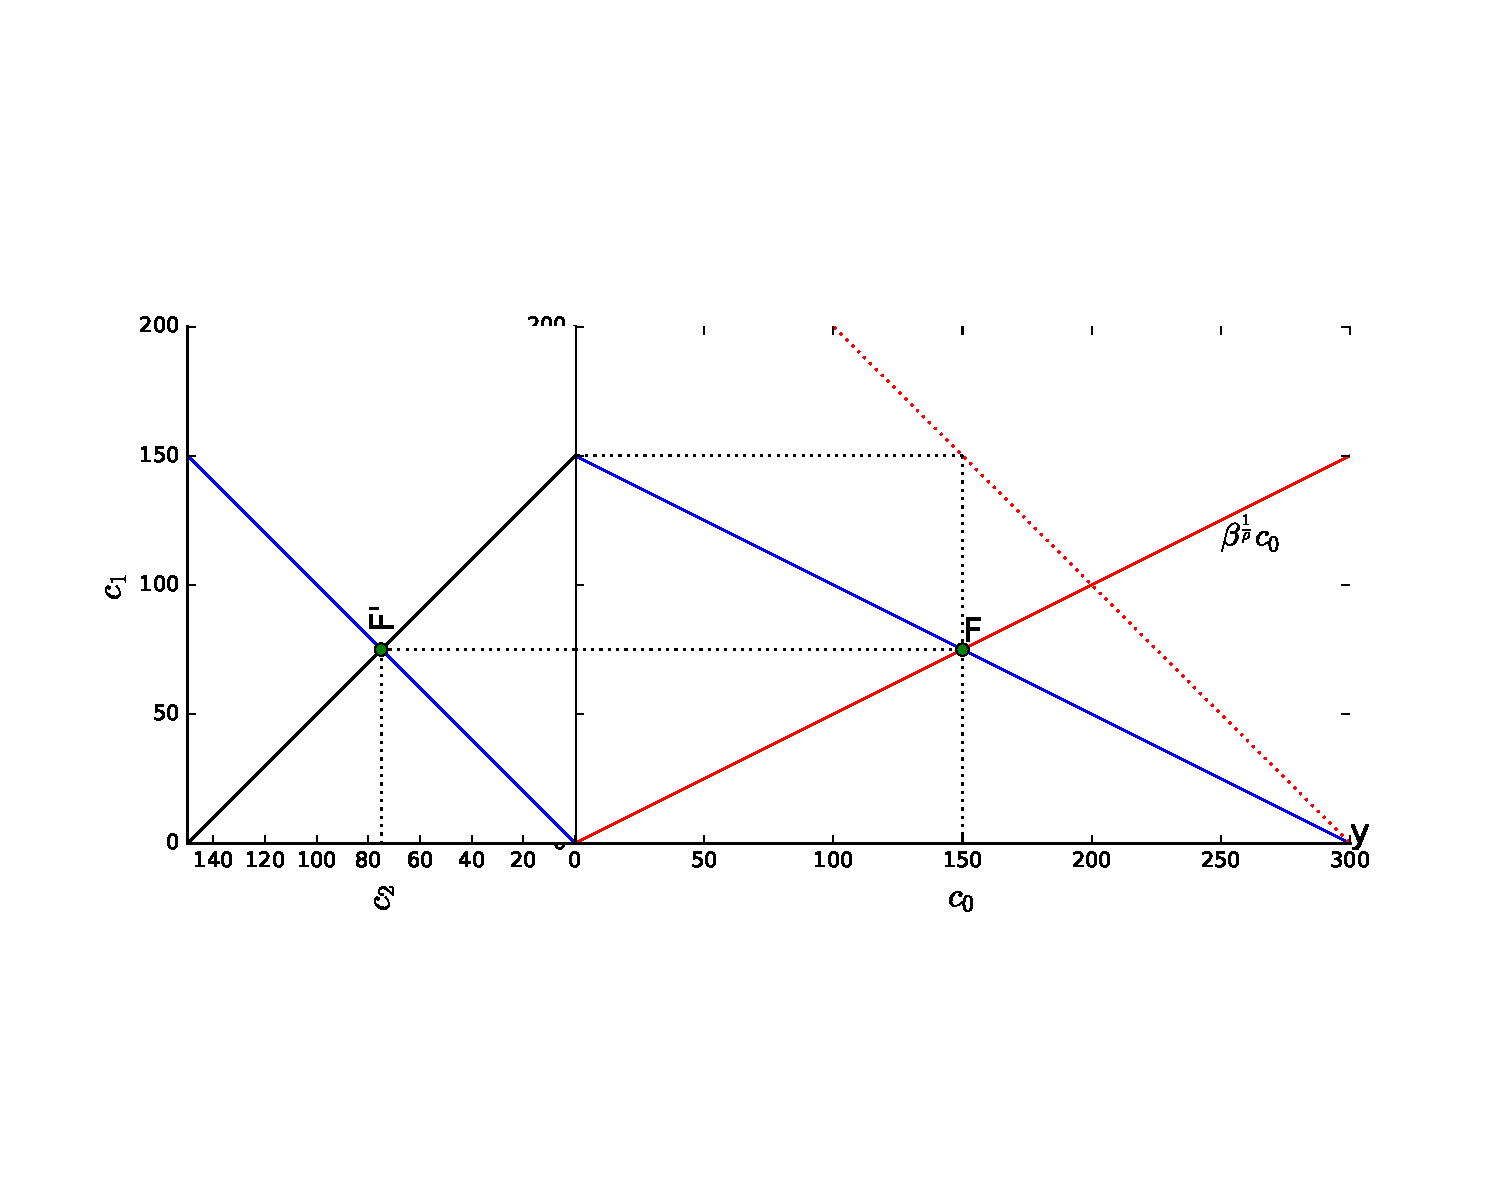
\includegraphics[clip,width=1\textwidth]{Figure1a.pdf}}

\subfloat[Renegotiation-proof with $\kappa=0$]{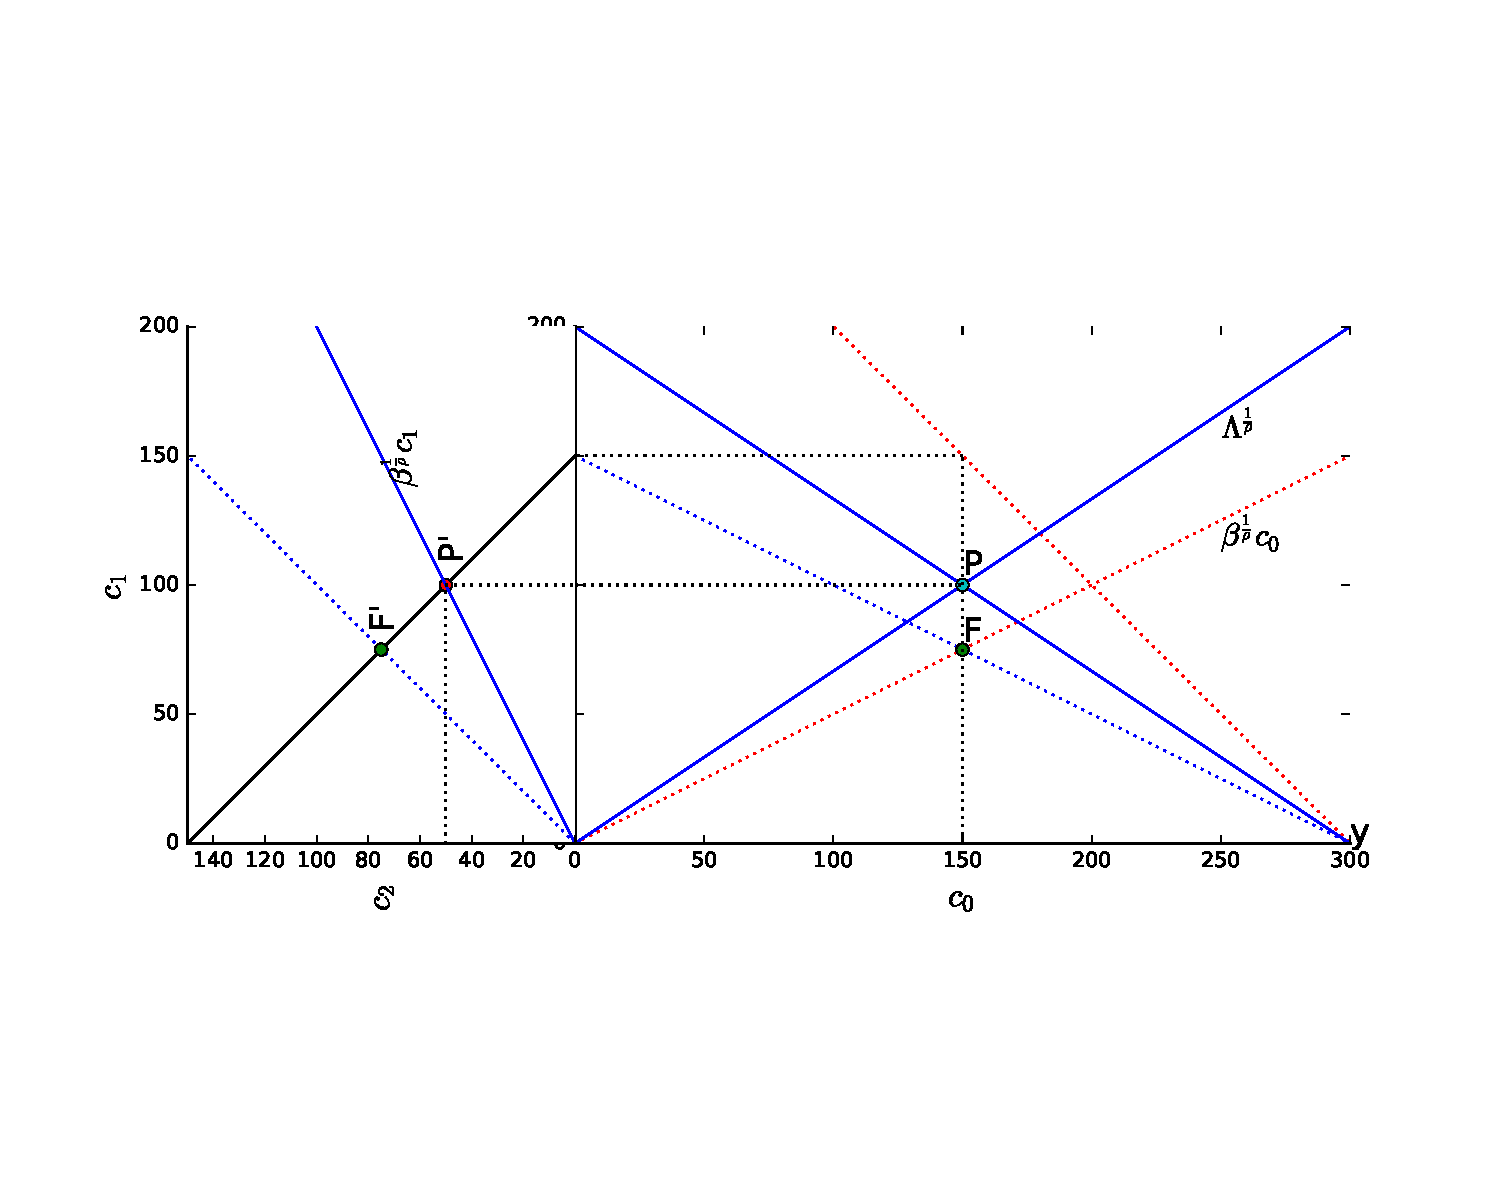
\includegraphics[width=1\textwidth]{Figure1b.pdf}}

\caption{Full-commitment and renegotiation-proof contracts under competition}

\label{fig:twoquad} 
\end{figure}

With an exclusive full-commitment contract the consumer faces no self-control
problem. Zero chooses a contract that commits her One- and Two- selves
to follow the chosen consumption plan. This contract design problem
is solved as a standard utility maximization problem subject to an
inter-temporal budget constraint (or subject to a financial intermediary's
zero-profit condition). Zero-self chooses contract $C_{0}$ to solve:
\begin{equation}
\max_{C_{0}}U_{0}(C_{0})\label{eq:cobj0}
\end{equation}
\begin{equation}
s.t.\quad\Pi_{0}(C_{0};Y_{0})\geq0\label{eq:BPC0}
\end{equation}
The familiar first-order necessary conditions are: 
\begin{equation}
u'\left(c_{0}\right)=\beta\delta(1+r)u'\left(c_{1}\right)=\beta\delta^{2}(1+r)^{2}u'\left(c_{2}\right)
\end{equation}

An increase or decrease to the term $\delta(1+r),$ which enters each
expression above, essentially `tilts' consumption to be more generally
rising or falling over time as $\delta\gtreqless1/(1+r)$. As this
across-the-board level of tilt will not alter key tradeoffs of interest
(unlike the degree of present-bias $\beta$ parameter which does)
we shall impose the assumption that $\delta=\frac{1}{1+r}$ for the
remainder of the analysis. This is without loss of generality but
will greatly unclutter the math. The simplified first-order conditions
are:
\begin{equation}
u'\left(c_{0}\right)=\beta u'\left(c_{1}\right)=\beta u'\left(c_{2}\right)\label{eq:FOC_comp}
\end{equation}

Along with a binding budget constraint the first-order conditions
allow us to solve for the optimal competitive `full-commitment' contract
$C_{0}^{F}$, so called because latter period selves are committed
to not change it. Conceptually the equilibrium contract will be found
at the tangency between the highest iso-utility surface just touching
the budget hyper-plane. With CRRA utility, a closed form solution
for $C_{0}$ is easily found which we label the competitive full commitment
contract $C_{0}^{F}$.\footnote{All CRRA derivations and closed-form solutions are in the appendix.}
This contract has the property: 
\[
c_{1}^{F}=c_{2}^{F}=\beta^{\frac{1}{\rho}}c_{0}^{F}
\]

Zero-self wants to indulge her present bias (by tilting consumption
toward herself) and then allocate remaining resources evenly across
the remaining two periods. 

This solution can be seen graphically in Figure 1a drawn for a consumer
with $\beta=0.5,$ $\rho=1$ and an intertemporal budget constraint
from endowment income with a present value of income $y=\sum y_{t}=300$.
The figure consists of two panels. The left panel depicts the $\left(c_{1},c_{2}\right)$
contract choice, conditional on $c_{0}=c_{0}^{F}$. The allocation
across periods 1 and 2 is determined by a budget constraint (the line
through $QF'$, satisfying $c_{1}+c_{2}=y-c_{0}$) and an optimal
`division rule' which in this case is $c_{1}=c_{2}$ (the line through
$OF'$). This division rule is attainable because full-commitment,
by definition, allows Zero-self to force One-self to respect the first-order
conditions of the maximization problem (\ref{eq:cobj0}).

The right panel depicts the $\left(c_{0},c_{1}\right)$choice conditional
on the division rule being followed in period 1. The budget constraint
(\ref{eq:budgetplus}) is the line going through $yF$ and the first-order
condition (\ref{eq:FOCc0c1}) is the line going through $0F$. 

The optimal contract $C_{0}^{F}$ lies at the intersections $F$ and
$F'$. To illustrate, at these parameters, Zero's preferred contract
is $C_{0}^{F}=(150,75,75)$. Whether the consumer borrows or saves
(or pays down debts) in any given period depends on how this consumption
stream matches her autarky consumption stream. If, for example, the
total income of $300$ arrives evenly across periods as $Y_{0}=(100,100,100)$
then this consumption plan would imply borrowing $c_{0}-y_{0}=50$
in period 0 to be repaid as installments of 25 in each of periods
1 and 2. If the stream had instead been $Y_{0}=(200,50,50)$ the consumer
would be seen as saving 50 in period 0 to raise consumption by 25
in each of periods 1 and 2.\footnote{These parameter values are chosen for expositional purposes. In particular
$\rho=1$ implies that period zero consumption will be the same with
or without self-control but the analysis can be easily adapted to
other cases.}

This approach will be useful for further analyzing situations where
Zero-self loses control over the division rule (i.e. loses commitment).

\subsubsection{Full-commitment contracts under Monopoly}

\label{sec:own}

If there is monopoly instead of competition for banking services in
period 0, the analysis is similar except that now we solve for the
optimum full-commitment contract by maximizing bank profits subject
to a consumer participation constraint. The bank solves: 
\begin{align}
\max_{C_{0}} & \;\Pi_{0}\left(C_{0};Y_{0}\right)\label{eq:monop-obj} \\
s.t. & \;U_{0}\left(C_{0}\right)\geq U_{0}^{A}(Y_{0})\label{eq:CPC0}
\end{align}

The first-order tangency conditions are the same as competitive case
given by expressions \ref{eq:FOC_comp}, which for CRRA utility again
implies $c_{1}=c_{2}=\beta^{\frac{1}{\rho}}c_{0}$. Along with the
fact that Zero's participation constraint must bind at a monopoly
optimum these equations allow us to solve for the contract $C_{0}^{mF}$
and corresponding bank profits $\Pi_{0}\left(C_{0}^{mF};Y_{0}\right)$.
Closed form solutions for the CRRA utility case appear as appendix
equations \ref{eq:c-mf} and \ref{eq:pi-mf}, respectively. Conceptually,
the optimum contract will be at the tangency point where the highest
iso-profit plane still touches the iso-utility surface associated
with Zero's reservation utility.

The terms of the optimal monopoly contract, and hence also the level
of bank profits achieved will be dependent on the consumer's autarky
utility $U_{0}^{A}(Y_{0})$. The present value of $C_{0}^{mF}$ rises
and profits fall with $U_{0}^{A}$. Since the monopolist retains the
gains from trade and consumer iso-utility (or indifference) surfaces
do not cross, consumption in each period under monopoly will be strictly
lower than under competition at all $Y_{0}$ except in the extreme
case where autarky utility is already optimal ($U_{0}^{A}=U_{0}^{F}$),
in which case the monopolist will trivially offer the utility maximizing
contract to the consumer and will make zero profits.

\section{The Renegotiation Problem}

We now get to the central questions of the paper: when is commitment
credible, how is it sustained, and at what cost? At issue is the fact
that One-self always prefers higher period 1 consumption than Zero
wants to build into a contract, so in any period 1 subgame between
One-self and the (same or a different) bank there will be tempting potential
gains to trade from breaking earlier contract commitments to Zero.
The credibility of the full-commitment contract must rest rest on
the threat of a sufficiently costly punishment deterring the bank
from engaging in such renegotiation. In this section we determine
the minimum size of the punishment required to deter the bank from
breaking the full-commitment contract.

The fraught nature of this potential renegotiation problem is depicted
in Figure \ref{fig:c1c2}, for a case where renegotiation costs are
set to $\kappa=0$. In other words, One-self and a bank are free to
costlessly rewrite the terms of any contract. Assume \textendash{}
just for the sake of argument now \textendash{} that the consumer
had (naively as it will turn out) accepted the a full commitment contract
$C_{0}^{F}$ or $C_{0}^{mF}$ in period zero, indicated as point $F$
in the figure. This contract satisfies Zero-self's optimality condition
$u'(c_{1})=u'(c_{2})$ as seen by the fact that Zero-self's indifference
curve is tangent to the bank's iso-profit line. For One-self's preferences
however this consumption bundle involves too little period 1 consumption
since $u'(c_{1})>\beta u'(c_{2})$ and as can be seen from the fact
that at $F$ One-self's indifference curve is steeper than the iso-profit
line. With zero renegotiation costs there are gains-to-trade that
can be shared from recontracting from $F$ to any new tangency point
(along the $c_{2}=\beta^{\frac{1}{\rho}}c_{1}$ ray where One-self's
first-order conditions are met) between point $R$ which is the contract
least favorable to One (chosen if the bank could act as monopolist
in period 1) and point $P$ which is the contract most favorable to
One (chosen with competitive refinancing). Zero is clearly worse off
with any such refinancing away from its preferred optimal contract
$F$.

 \begin{figure}
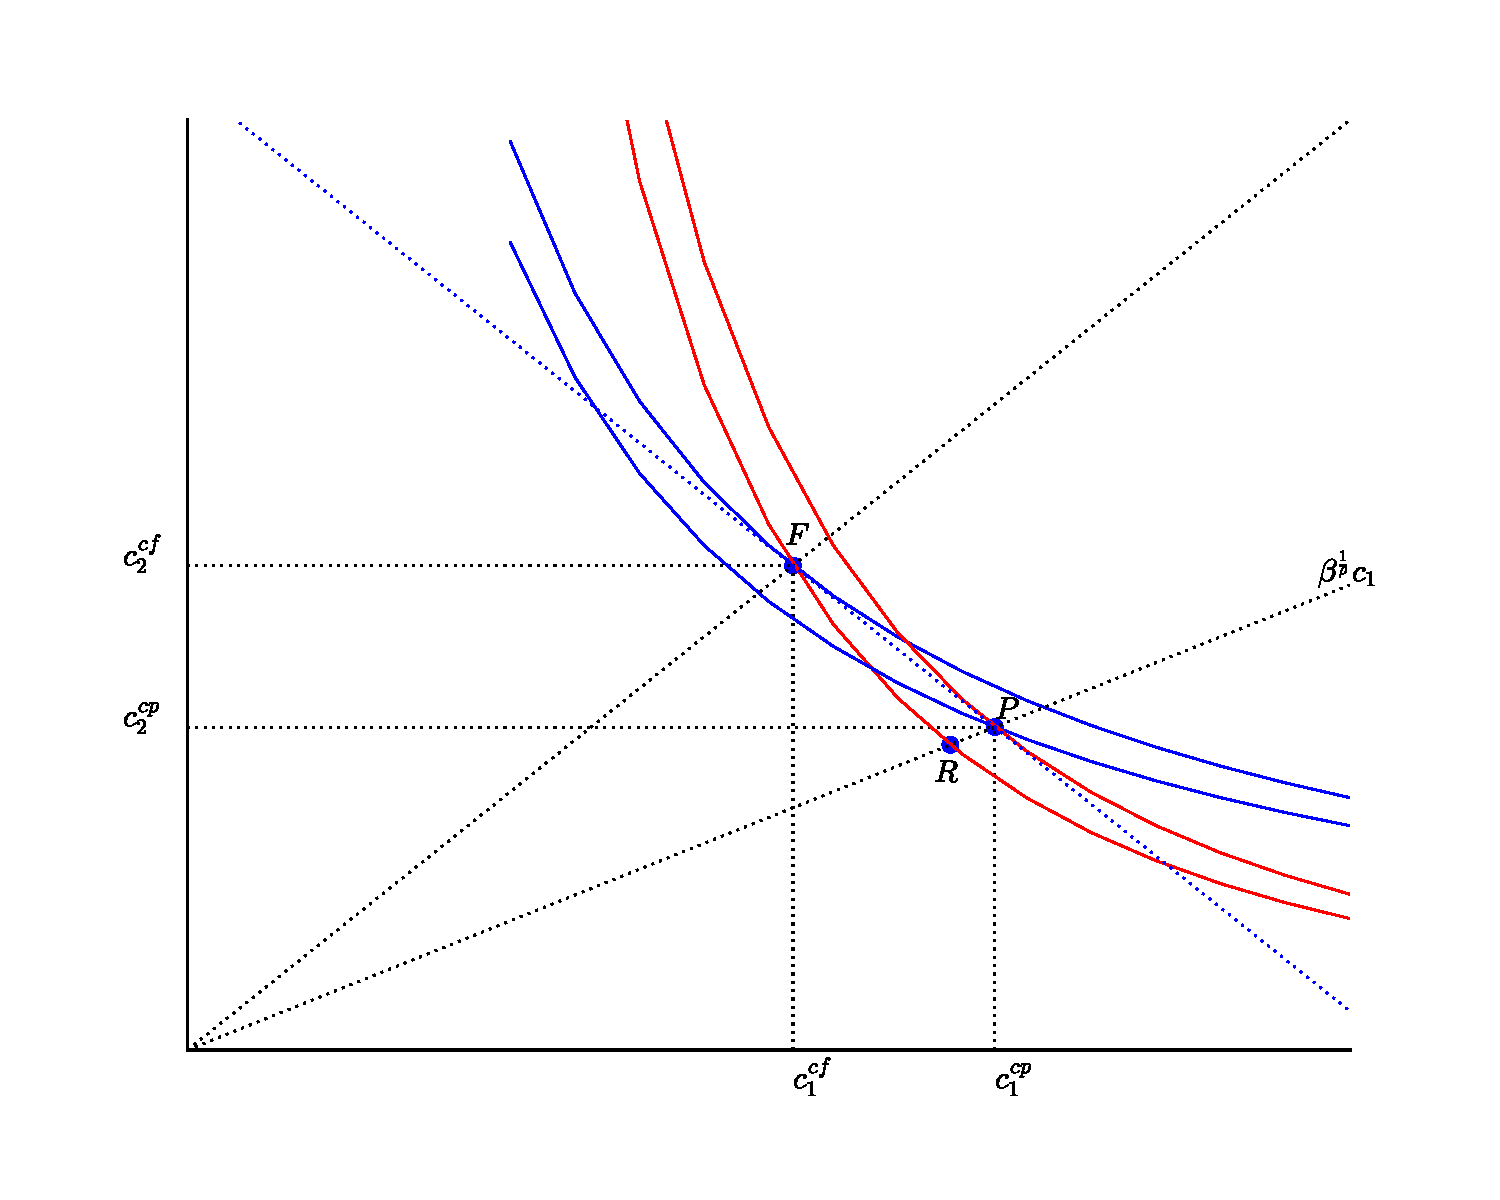
\includegraphics[width=\textwidth]{fig_selfcontrol.pdf}
\caption[Full-commitment and renegotiation-proof contracts under competition]{Full-commitment and renegotiation possibilities in period 1
 (drawn for \\ $c_{0}=c_{0}^{F},\beta=\frac{1}{2},\rho=1,\kappa=0$)}

\label{fig:c1c2}
\end{figure}

\subsection{Renegotiated contracts}

Consider the subgame entered in period 1, with $C_{1}^{0}=(c_1^0,c_2^0)$ denoting
the terms of any continuation contract inherited from period 0. We
now formally derive conditions under which the contract will survive
the threat of renegotiation in period 1. Below, we characterize the
`best response' contract chosen in the subgame of period 1, conditional
on the contract being renegotiated. Note that the terms of the renegotiated
contract and therefore also the division of the gains to trade will
depend on the period 1 market for refinances is competitive or monopolized
(or something in between). The contract will be renegotiated if the
gains to trade are sufficient to cover the bank's renegotiation costs
$\kappa$.

Consider first the situation where the market for refinanced contracts
is competitive (i.e. the period 0 bank cannot enforce an exclusive
contract). For the present analysis it turns out that it does not matter whether there
was competition or monopoly in period 0. Competition in period 1 will
lead banks to offer to renegotiate the existing continuation contract
$C_{1}^{0}$ for a new contract $C_{1}^{1}(C_{1}^{0})$, allowing
the (new or existing) bank to just break even after covering any renegotiation
costs: 
\[
C_{1}^{1}(C_{1}^{0})=\arg\max_{C_{1}}\ U_{1}(C_{1})
\]
\begin{equation}
\Pi_{1}(C_{1};C_{1}^{0})\ge\kappa\label{eq:PiGain}
\end{equation}
As long as $U_1$ is well behaved this can be solved for an interior $C_{1}^{1}(C_{1}^{0}) $ using the first-order condition $u'(c_1^1)=\beta u'(c_2^1)$ and the binding condition \ref{eq:PiGain}.   As drawn in figure ?? for the CRRA case (\ref{eq:c-r}),
the contract $C_{1}^{0}$ at \textbf{P} would be renegotiated to point \textbf{$R(\kappa)$} where the ray $c_{2}^{1}=\beta^{\frac{1}{\rho}}c_{1}^{1}$ (along which the FOA are met) intersects the period 1 zero profit line  \ref{eq:PiGain}.
One-self makes a utility gain. Note that had $\kappa=0$ the contract would have been renegotiated to \textbf{$R(0).$}

If the bank instead finds itself in a monopoly position in period
1 then it will renegotiate existing contract $C_{1}^{0}$ to a new
contract $C_{1}^{m1}(C_{1}^{0})$ to increase profits by offering
the smallest possible enticement for One-self to accept the renegotiated
contract.

\[
C_{1}^{1m}(C_{1}^{0})=\arg\max_{C}\ \Pi_{1}(C_{1};C_{1}^{0})
\]
\begin{equation}
U(C_{1})\geq U(C_{1}^{0}) \label{eq:ugain}
\end{equation}
Solving for an interior solution using first-order conditions and the binding condition \ref{UGain}, the CRRA case yields a closed form solution (\ref{eq:m-r}). In figure ?? contract $C_{1}^{0}$ at \textbf{P} would be renegotiated to point \textbf{$R^{m}$} where the ray $c_{2}^{1}=\beta^{\frac{1}{\rho}}c_{1}^{1}$ intersects One-self's participation constraint  \ref{eq:PiGain}.
As drawn the bank gains. \subsection{The `no-renegotiation' condition}

Under what conditions would the original contract \textit{not} be
renegotiated in period 1? Assuming a tie-breaking rule in favor of
Zero-self's preferences, the no-renegotiation condition under period
1 competition is:
\begin{equation}
U_{1}\left(C_{1}^{0}\right)\geq U_{1}\left(C_{1}^{1}(C_{1}^{0})\right)\label{eq:no-reg-comp}
\end{equation}

And the no-renegotiation condition under period 1 monopoly is:
\begin{equation}
\Pi_{1}(C_{1}^{1}\left(C_{1}^{0}\right);C_{1}^{0})\leq\kappa\label{eq:no-reg-monop}
\end{equation}

Notice that these two conditions are in fact identical: a period 0 contract
is credible if and only if there is no way for a bank to offer One-self
a new contract that simultaneously (a) leaves One-self with at least
as much discounted utility as in the original contract, and (b) generates
additional profits of at least $\kappa$ to the bank. In short the contract is renegotiation-proof as long as renegotiation costs are large enough to make sure no Pareto-gain is possible between One-self and the bank. This results
in a single no-renegotiation condition that can be applied to any
contract $C_{1}^{0}$ and renegotiation cost $\kappa$ (a closed-form
solution representation is given in Equation \ref{eq:no-renegotiation}).

This condition can be illustrated using Figure \ref{fig:c1c2}. Let
$F$ denote \textit{any} inherited contract in period 1. The horizontal
distance between the isoprofit lines through $P$ and $R$ denotes
the maximum possible profit gains a bank could earn through renegotiation (equal to  the cost savings from renegotiating the contract $c_1^0+c_2^0 -c_1^1-c_2^1$.
So, if this distance is less than or equal to $\kappa$, the consumer
and the bank will not find it worthwhile to renegotiate.

\subsection{At what cost are full-commitment contracts kept credible?}

Now, we turn to the survival of full-commitment contracts in particular.
What minimum renegotiation cost is sufficient to deter the renegotiation
of full-commitment contracts? This is easily derived by setting $c_{1}^{0}=c_1^F=c_{2}^{0}$
in the no-renegotiation condition (\ref{eq:no-renegotiation}). A
competitive full-commitment contract will survive if and only if
\begin{equation}
\kappa\geq\bar{\kappa}\equiv c_{1}^{F}\cdot \Upsilon
\end{equation}
and a monopolistic full-commitment contract will survive if and only
if:
\begin{equation}
\kappa\geq\bar{\kappa}^{m}\equiv  c_{1}^{mF} \cdot \Upsilon
\end{equation}
where 
\begin{equation}
\Upsilon =\left(2-\left(\frac{1+\beta}{\left(1+\beta\right)^{\rho}}\right)^{\frac{1}{1-\rho}}\right)\label{eq:kbar}
\end{equation}
$\bar{\kappa}$ and $\bar{\kappa}^{m}$ are the minimum renegotiation
costs required for the survival of full-commitment contracts. These
conditions tell us that, the greater the consumption levels in a full-commitment
contract, the harder it will be to avoid renegotiation (i.e. the greater
is the scope for rearranging consumption profitably in period 1.)

The value of $c_{1}^{0}$ in the expression will be different depending
on whether the period 0 market for full-commitment contracts is competitive
or monopolized. Under competition from \ref{eq:CF} and \ref{eq:CF1}
we know that $c_{1}^{F}=\frac{\beta^{\frac{1}{\rho}}y}{1+2\beta^{\frac{1}{\rho}}}$.
Since this does not depend on autarky utility (given a fixed value
of $y$), $\bar{\kappa}$ too does not depend on how close or far
to optimal consumption smoothing the consumer is in autarky.

If the market for period 0 full-commitment contracts is monopolized
we are led to a cutoff $\bar{\kappa}^{m}$ that now depends on autarky
utility. The higher is $U_{0}^{A}(Y_{0})$ the higher will be $c_{1}^{mF}$.
Since $c_{1}^{F}\ge c_{1}^{mF}$ for any initial $Y_{0}$ it must
be the case that $\bar{\kappa}^{m}\le\bar{\kappa}$. 

Together, this indicates that, if renegotiation costs lie above cutoff
$\bar{\kappa}$, full commitment contracts will be credible; and if
renegotiation costs lie below this cutoff, the survival of full-commitment
will depend on market structure and autarky utility. Proposition 1
summarizes the results.
\begin{prop}
Consider renegotiation costs $\bar{\kappa}$ and $\bar{\kappa}^{m}$
as defined in Conditions \ref{eq:kbar} and \ref{eq:kbar-m}.

(a) The competitive full commitment contract survives if and only
if $\kappa\geq$$\bar{\kappa}$.

(b) The monopolistic full commitment contract survives if and only
if $\kappa\geq$$\bar{\kappa}^{m}$. $\bar{\kappa}^{m}$ is strictly
rising in the consumer's autarky utility.

(c) $\bar{\kappa}^{m}\leq\bar{\kappa}$.
\end{prop}
Note that the monopolist's ability to commit at lower threatened renegotiation
cost ($\bar{\kappa}^{M}\le\bar{\kappa}$) comes from the fact that
its commitment contract is less susceptible to renegotiation. That
is because, having, at the outset, extracted surplus by offering the
consumer a contract with the lowest possible consumption, there is
relatively less for the firm to capture via renegotiation in period
1. This stands in contrast to the intuitive notion that a monopolist
might offer better commitment because it faces greater costs of breaking
promises than a competitive firm does. Our result shows that even
in the absence of this mechanism, monopoly contracts are inherently
harder to break.

A further implication, of statement (b) in the proposition, is that
under monopoly, consumers with already relatively smooth consumption
are less likely to get full-commitment contracts that can be sustained.
A consumer with a higher autarky utility must be offered higher consumption
by the monopolist. And the no-renegotiation condition is harder to
satisfy at higher levels of consumption.


\section{Imperfect Commitment Contracts }

\label{sec:imperfectK}

We turn now to situations where
 renegotiation costs $\kappa$ are positive but not sufficiently large to sustain full-commitment contracts.  So long as   One self's  consumption tradeoffs differ from Zero's renegotiation  can only harm (or, at best, not improve) Zero-self's inter-temporal welfare.      In the case of naifs, banks will
capitalize on the consumer's failure to anticipate harmful renegotiation (Section 4.4). In the case of sophisticates, the   Zero-self consumer will seek to avoid entering into multi-period contracts that are vulnerable to such harmful renegotiations. They will limit their  choice to contracts that are  renegotiation-proof or subgame-perfect (Sections 4.2 and 4.3).  If renegotiation-proof constraint \ref{eq:no_reneg} binds at an optimum the resulting  optimal contract will offer less consumption smoothing than the full-commitment contract. The absence of a sufficiently tough external deterrent  to renegotiation leads the parties to build what commitment they can by tilting the terms of the period 1 continuation contract closer to One-self's
preferences so as a way to reduce the scope for renegotiation. 
We call these `imperfect commitment' contracts. These are still commitment contracts -- renegotiation is avoided in equilibrium-- but at the cost of now less than perfect consumption smoothing for Zero. 

\section{Renegotiation-proof contracts with $(0\leq\kappa<\bar{\kappa})$ }

We turn now to the multi-period contract design problem between a sophisticated consumer and a bank in period 0 when bank renegotiation costs are not sufficient to sustain full-commitment contracts. We take renegotiation costs to be exogenously given.\footnote{In later sections we explore costly endogenous strategies to shape perceptions of renegotiation costs and competition across banks with differing levels.} There are two cases to consider: when the market for period 0 contracts is competitive and when it is monopolized. 

\subsection{Competitive renegotiation-proof contracts}

If the period 0 market is competitive and the market for period 1 renegotiated contracts is expected to be a monopoly (i.e. an enforceably exclusive contract)\ the optimum contract
will solve the following problem:

\begin{align}
 & \max_{C_{0}}\ U_{0}\left(C_{0}\right)  \tag{\ref{eq:cobj0}} \\
 & \ \ \Pi_{0}\left(C_{0};Y_{0}\right)\geq 0 \tag{\ref{eq:BPC0}} \\
 & \ \ \Pi_{1}\left(C_{1}^{1}\left(C_1^0\right);C_{1}^0\right)
 \leq\kappa\tag{\ref{eq:no-reg-monop}} 
\end{align}
If we instead the Zero-self consumer had expected the period 1 market for renegotiated contracts to be competitive then we would have had the same objective and period 0 bank participation constraint but we would have replaced the period 1 bank no-renegotiation constraint \ref{eq:no-reg-monop} with a no-renegotiation constraint on One-self:
\begin{align}
U_{1}(C_1^1(C_1^0)) \le U_{1}(C_1^0) \tag{\ref{eq:no-reg-comp}}
\end{align}
However, as we have alluded to already and explain again below  in either case -- whether the period 1 market for renegotiated contracts is a monopoly or competitive -- both constraints \ref{eq:no-reg-comp} and \ref{eq:no-reg-monop} will bind at an optimum.

Similar to a Stackelberg leader choosing the most favorable of possible market outcomes along their opponents reaction function in a Cournot duopoly game, Zero-self  will choose the contract $C_0^0$ that offers the highest welfare considering the  strategic game play between the bank and One-self in the period 1 subgame $\zeta(C_1^0,\kappa)$. 


Figure \ref{fig:compRP}\ is useful for understanding expected game play in for different  subgames $\zeta(C_1^0,\kappa)$ in period 1. The figure is  zoomed in around the contract space of interest to make the relationships clearer.
Suppose Zero-self has chosen a candidate level of period 0 consumption $c_1^0$. For this to be part of an optimum contract Zero must insure that its continuation contract $C_1^0=(c_1^0,c_2^0)$ lies on the bank's binding period 0 zero profit condition (or else Zero-self can raise her welfare could be made higher ). This is equivalent to stating that the continuation contract will lie along the period  1 budget line $c_1^0+c_2^0=y-c_0^{0}$ drawn running through point $R(0)$ in the figure.   
 
 Note that a bank will only accept to renegotiate away from a  contract on this budget line if the renegotiated contract $(c_{1},c_{2})$ lies on or below iso-cost line $c_1+c_2 =y-c_0^0-\kappa$ because by design any contract above this line cannot offer sufficient cost savings (i.e. profit gains) to cover renegotiation cost $\kappa$. We also know from our earlier analysis of best renegotiation offers (recall our derivation of $C_1^1(C_1^0)$ and $C_1^{m1}(C_1^0)$ ) that candidate renegotiation contracts must satisfy One's first order condition $u'(c_1)=\beta u'(c_2)$ -- otherwise the gains to trade from renegotiation could be increased to make these renegotiation more attractive. The unique contract that just satisfies these two conditions -- the most attractive renegotiation that is just rejected -- is  represented by $R(\kappa)$.\footnote{With period 0 is competitive we'll have $c_1^0+c_2^0=y-c_0^0$ and can therefore identify this point from $u'(c_1)=\beta u'(y-c_0^0-\kappa-c_1)$. For the CRRA case $c_1=(y-c_0^0-\kappa)/(1+\beta^\frac{1}{\rho})$}  

\begin{figure}
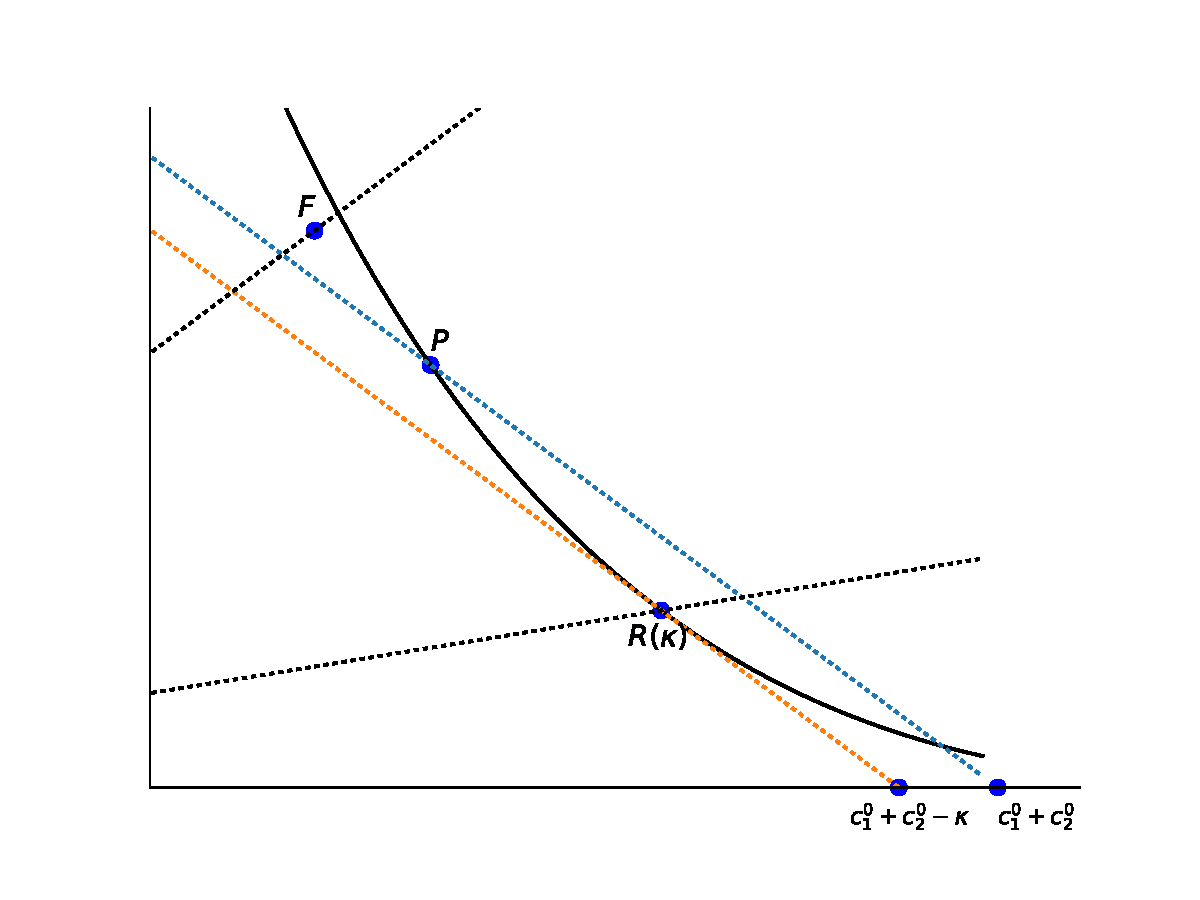
\includegraphics[width=\textwidth]{CompetitiveRP.pdf}

\caption{Competitive commitment contract with $\kappa < \bar \kappa$}
\label{fig:compRP}
\end{figure}

Now draw  an indifference curve  for One-self's preferences through this point. All points on the period 1 budget line $c_1^0+c_2^0=y-c_0^0$ that also lie above this indifference curve will be renegotiation-proof contracts. \ To see this consider any contract $P'$ on this segment. One-self will only accept renegotiation away from this  contract if it moves One-self to an indifference curve just above the one running through $P'$ but, by construction, any such contracts clearly lie above the bank's no-renegotiation  and hence would be rejected.  By similar reasoning any contract along the budget line  outside of this segment would be renegotiated. Zero-self's welfare rises as we move to more balanced consumption bundles along this line so Zero's preferred renegotiation-proof contract will be the contract labeled $P$ in the diagram. For all $\kappa<\bar \kappa$ the so chosen optimal renegotiation-proof contract will offer less consumption and hence lower welfare compared to the full commitment contract (reached at $\kappa=\bar \kappa$).

Mathematically, for $c_0^0$ given the best continuation contract is found using three equations. Bank no-renegotiation condition $c_1^1+c_2^1=y-c_0^0-\kappa$ and first order condition $u(c_1^1)=\beta u(c_1^2)$ to solve for best renegotiation offers $c_1^0$ and $c_2^0$ as a function of pre-determined $y,c_0^0$ and $\kappa$, and One-self no-renegotiation condition  $u(c_1^0)+\beta u(c_2^0)=u(c_1^1)+\beta u(c_2^1)$ and One's first-order condition to then solve for the optimal continuation $c_1^0$ and $c_2^0$ as a function of  those same pre-determined variables.  Using this method to find the best continuation contract for candidate $c_0^0$ Zero-self can now search over all candidate $c_0^0$ to find the welfare maximizing three-period contract. 

However, except for the special case where $\kappa=0$ described below, 
 there will be no simple closed form solution for the optimal contract even in the CRRA\ case. This can be seen from the fact that there are in fact two points where the no-renegotiation condition indifference curve crosses the period 1 zero-profit line. As described in the appendix for the\ CRRA\ case the  c_1^0$ coordinates of these two roots are given by the following non-linear equation:

\begin{equation}
 u(c_1^0)+\beta u((y-c_0^0) - c_1^0) = (1+\beta^\frac{1}{\rho}) u \left(\frac{y-c_0^0 - \kappa}{1+\beta^\frac{1}{\rho}}\right) 
\end{equation} 
  

 
\subsection{The competitive case when $\kappa=0$ }

In the special case of perfect competition with costless renegotiation ($\kappa=0$) the above equation has just one solution. In terms of figure \ref{fig:compRP} think of how $P$ would slide down the period 1 budget line as $\kappa$ shrinks until we get to a point where One's indifference curve is just tangent to the period 1 budget line.   This continuation contract is 'renegotiation-proof' but only in the very narrow sense that it won't be renegotiated because it already delivers One-self's preferred consumption choice.

The left panel the lower Figure 1b has figure \ref{fig:compRP} rotated counter-clockwise 90 degrees in order to show how Zero self's strategic choices will be made in $c_0-c_1$ space in the right panel. In contrast to Figure 1a where $\kappa>\bar \kappa$ and where One-self can be credibly committed to dividing consumption resources equally between periods 1 and
2, when $\kappa=0$  
that division would always be renegotiated in ways harmful to Zero. Being a sophisticate, Zero understands that the only way  to avoid renegotiation is to satisfy One's period 1 first-order condition $u'(c_1^0)=u'(c_1^0)$. For the CRRA case depicted these FOCs are indicated by the dashed line though $OP'$ (or $c_{2}=\beta^{\frac{1}{\rho}}c_{1}$) in the
left panel.

One's best response function to Zero's period 0 consumption choice is given by the tangency between One-self's indifference curve and the period 1 budget line $y-c_0^0$ which can be easily solved to give:
\begin{align}
c_{1}^{1}(c_{0}) & =\frac{y-c_{0}}{1+\beta^{\frac{1}{\rho}}}\label{eq:react1}\\
c_{2}^{1}(c_{0}) & =\beta^{\frac{1}{\rho}}\cdot c_{1}^{1}(c_{0})\label{eq:react2}
\end{align}
This subgame reaction function can be visualized as the line passing through
$yP$ in the right panel of Figure \ref{fig:twoquad} (from expression
\ref{eq:react1})\ and the line passing through $OP'$ in the left
(from \ref{eq:react2}).

Being sophisticated, Zero anticipates her future self's reaction and
strategically chooses $c_{0}^{\ensuremath{}}$ to solve: 
\begin{equation}
\max_{c_{0}}u(c_{0})+\beta[u(c_{1}^{1}(c_{0})+u(c_{2}^{1}(c_{0})]
\end{equation}
subject to the bank's period 0 participation (or zero-profit) constraint:
\begin{equation}
c_{0}+c_{1}^{1}(c_{0})+c_{2}^{1}(c_{0})=y
\end{equation}
From the fact that One wants to set $c_{2}^{1}=\beta^{\frac{1}{\rho}}c_{1}^{1}$
and other substitutions the first-order condition for this problem
can be written: 
\begin{align}
u'(c_{0}) & =\Lambda u'(c_{1})\nonumber \\
\text{ or }c_{1} & =\Lambda^{\frac{1}{\rho}}c_{0}\label{eq:LambdaC0}
\end{align}
where 
\begin{equation}
\Lambda=\frac{(\beta+\beta^{\frac{1}{\rho}})}{1+\beta^{\frac{1}{\rho}}}
\end{equation}
Equation \ref{eq:LambdaC0} defines the line passing through OP.

Zero self
chooses the consumption contract along subgame reaction function that
places her on the highest possible iso-utility surface. The equilibrium
contract $P$ satisfies both equation \ref{eq:react1} (the line through
yP) and equation \ref{eq:LambdaC0} (the line through OP). These equations
can be solved to yield the closed-form solution to the optimal contract
\begin{equation}
c_{0}^{P}=\frac{y}{1+\Lambda^{\frac{1}{\rho}}(1+\beta^{\frac{1}{\rho}})}\label{eq:coP}
\end{equation}
with $c_{1}^{P}=\Lambda^{\frac{1}{\rho}}c_{0}^{P}$ and $c_{2}^{P}=\beta^{\frac{1}{\rho}}\Lambda^{\frac{1}{\rho}}c_{0}^{P}$.

It is easy to check that $\Lambda>\beta$ for all $0<\beta<1$ and
hence line $OP$ is everywhere steeper than line $OF$. Combined with
our earlier observation that line $yP$ is everywhere steeper than
line $yF$ we conclude that $c_{1}^{P}>c_{1}^{F}$ over the same parameter
range. Hence, the inability to enforce commitment leads to higher
consumption in period one compared to a situation where it can be
enforced. The subgame-perfect `renegotiation-proof' contract will
involve less net saving (or equivalently, more net debt) in period
1 than Zero self would like (as can be seen by $u'(c_{1}^{P})<u'(c_{2}^{P})$)
and lower Zero self welfare compared to the full-commitment contract.

To illustrate, at our earlier parameterization $\beta=0.5$ and $\rho=1$
the full commitment contract will be $C_{0}^{P}=(150,100,50)$ which
offers considerably less consumption smoothing in later periods compared
to the contract with self-control $C_{0}^{F}=(150,75,75)$. If the
consumer's initial income stream were $Y_{0}=(100,100,100)$ then
we could think of the consumer with self-control as sticking to a
balanced repayment program to keep consumption steady in the last
two periods. Compared to this the consumer without self-control rolls
over debt rather than repay it in period one. The entire burden of
repayment of the debt that Zero took out in period 0 now falls in
period 2, whereas Zero would have preferred the burden to be shared
equally between periods 1 and 2. If the income stream had instead
been $Y_{0}=(200,50,50)$ then a consumer without self-control would
be viewed as raiding savings in period 1 that an otherwise identical
consumer with self-control would have earmarked for period 2 consumption.
In short, consumers that can obtain full-commitment contracts will
save/repay more or borrow less in period 1 and consume more in period
2 and the inability to do so leads to lower welfare for Zero in this
competitive setting.

More generally, if $\kappa$ is small but non-zero, then Zero-self
is not entirely bound to One-self's preferences. Credible division
rules between periods 1 and 2 depend on the no-renegotiation constraint
in some subtle ways. In the following sections, starting with monopoly,
we show how the contract terms change in such cases.


\subsection{Monopoly renegotiation-proof contracts}

When the market for period 0 contracts is monopolized the analysis is broadly similar to the competitive case above, with some wrinkles.  The monopoly bank will want to maximize multi-period profits (objective \ref{eq:monop-obj}) subject to Zero-self's participation (constraint \ref{eq:CPC0}) and the constraint that continuation contracts be renegotiation proof (i.e. no-renegotiation constraints \ref{eq:no-reg-comp} and \ref{eq:no-reg-monop} both hold).  




A sophisticated consumer
can rationally anticipate how her
later self may be tempted to renegotiate. Zero-self would agree to a contract that will be renegotiated  but only if the bank adjusts the terms of the offered period 0 contract to compensate for the reduced consumption smoothing that would result.  This however can only harm bank profits as the cheapest to satisfy Zero's participation constraint is by offering consumption smoothing. Hence the monopoly bank will itself insist on renegotiation-proof contracts.       


\begin{figure}
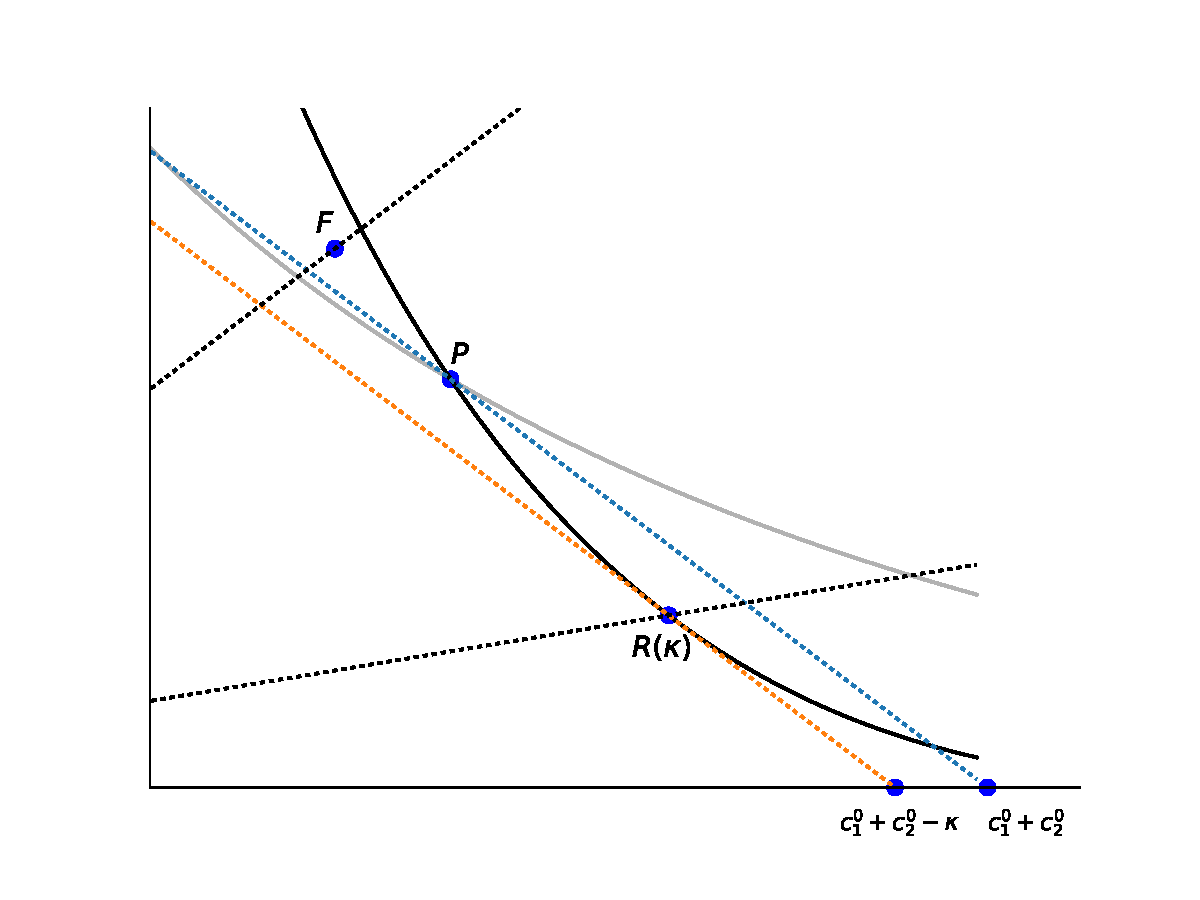
\includegraphics[width=\textwidth]{MonopolyRP.pdf}

\caption{Monopoly commitment contract with $\kappa < \bar \kappa$}
\label{fig:monopRP}
\end{figure}

The bank will be looking for the most profitable renegotiation-proof contract that lies on Zero's participation constraint \ref{eq:CPC0}. If the bank has chosen candidate contract $C_0^0$ then the bank an optimum continuation contact $C_1^0=(c_1^0, c_2^0)$ must lie along Zero's autarky utility surface which can be projected as indifference curve $\beta \left [u(c_1^0)+u(c_2^0) \right]=U_0^A-u(c_0^0)$ in $c_1-c_2$ space. The optimal contract will be the most profitable renegotiation proof contract along this surface. The contract will be renegotiation proof when $c_1^1+c_2^1+\kappa \ge c_1^0 +c_2^0$ and $u(c_1^1)+\beta u(c_2^1)\le u(c_1^0)+\beta u(c_2^0)$. Many points are renegotiation proof but the one that is most profitable amongst these will satisfy the two conditions exactly depicted in the figure by point $P$.  

The renegotiation-proof contract can be explicitly
derived for the CRRA case of $\kappa=0$ (Equation \ref{eq:zerokappa-monop}).
For, $\kappa>0$, the contract cannot be explicitly derived in closed
form, but its key properties can be established. 
\begin{prop}
Suppose $\kappa<\bar{\kappa}$. If $U_{0}^{A}\leq U^{m}$, the bank
offers the full-commitment contract $C_{0}^{mF}$. If $U_{0}^{A}>U^{m}$,
the bank offers the renegotiation-proof contract $C_{0}^{mP}$, and:

(a) $\Pi_{0}\left(C_{0}^{mP};Y_{0}\right)<\Pi_{0}\left(C_{0}^{mF};Y_{0}\right)$

(b) There is some $\bar{U}\epsilon\left(U^{m},U_{0}^{F}\right)$ such
that, if $U_{0}^{A}>\bar{U}$, the bank would earn negative profits
and therefore will not offer a contract.

(c) $c_{0}^{mP}>c_{0}^{mF}$. 
\end{prop}
Proposition 2 compares the renegotiation-proof contract to the full-commitment
contract when the renegotiation-proofness constraint binds. Part (a)
states that bank profits will be lower than under full-commitment.
The bank wishes it could promise to not renegotiate but it cannot
make such a promise credible without giving up some profits. The problem
here is not one of cheating or contract failure (as examined for example
by Hansmann (1980) and Glaeser-Shleifer (2001)), it is the possibility
of a legitimate renegotiation (a voluntary agreement to tear up the
old contract) between the consumer and the firm. The monopolist would
have gained from having higher renegotiation costs since in equilibrium
renegotiation does not take place.

Part (b) follows from part (a). If the bank were able to provide full
commitment, it could offer a profit-making contract to any individual
with even minimal smoothing needs. Now however, for individuals whose
autarky utility is close enough to $U_{0}^{F}$, the bank would make
negative profits and therefore no contract is offered to them. This
is because the renegotiation-proofness constraint may require even
greater imbalance in consumption across periods 1 and 2 than under
autarky.

Part (c) is about the terms of the contract itself\textendash when
full-commitment is not feasible, the renegotiation-proof contract
will involve higher consumption in period 0 (i.e. either a smaller
loan or less savings) compared to full commitment. The following is
a sketch of the argument. Let the full-commitment contract be described
by some $c_{0}=c_{0}^{mF}$ (period 0 consumption) and $s=s^{mF}$
(sum of $c_{1}$ and $c_{2}$, which are equal in size). Since the
full-commitment contract lies at an optimum, it must be true that
at the levels of consumption specified by the contract, the marginal
utility of present consumption is equal to the discounted marginal
utility of future consumption: 
\begin{equation}
\frac{du\left(c_{0}^{mF}\right)}{dc_{0}}=\frac{d\left(\beta u\left(\frac{s^{mF}}{2}\right)+\beta u\left(\frac{s^{mF}}{2}\right)\right)}{ds}
\end{equation}
Now suppose $c_{0}^{mP}=c_{0}^{mF}$, so that period 0 consumption
in the renegotiation-proof contract is held the same. Since any future
consumption will be split unevenly, in order to continue to satisfy
the consumer's period 0 participation constraint, it must be true
that $s^{mP}>$$s^{mF}$. We show in the appendix that $s^{mP}$ will
be large enough that, at these values,
\begin{equation}
\frac{du\left(c_{0}\right)}{dc_{0}}>\frac{d\left(\beta u\left(c_{1}\left(s\right)\right)+\beta u\left(c_{2}\left(s\right)\right)\right)}{ds}
\end{equation}
So the bank can do better by raising period 0 consumption at the expense
of future consumption. The bank limits renegotiation possibilities
by transferring consumption away from the future (when renegotiation
is a temptation) to the present.

To summarize: the requirement that contracts be renegotiation-proof
results in higher period 0 consumption and lower bank profits, and
the denial of service (rationing) of consumers whose smoothing needs
are relatively small.

\subsection{Competition with $\kappa>0$}

As mentioned earlier, under competition, the terms of a renegotiated
contract depend on exclusivity but the no-renegotiation constraint
does not. So, regardless of exclusivity, the equilibrium contract
under competition is given by:\footnote{A similar analysis could be conducted even if the costs of renegotiating
another bank's contract are different from $\kappa$, the costs of
renegotiating one's own contract.}

\begin{align}
 & \max_{C_{0}}\ U_{0}\left(C_{0}\right)\nonumber \\
 & s.t.\ \Pi_{0}\left(C_{0};Y_{0}\right)\geq0\label{eq:bpc-rp}\\
 & \Pi_{1}\left(C_{1}^{m1}\left(C_{1}\right);C_{1}\right)\leq\kappa\label{eq:rpc-c}
\end{align}

This yields a contract $C_{0}^{P}$. Given our assumption that $\kappa<\bar{\kappa}$,
the renegotiation-proofness constraint (\ref{eq:rpc-c}) binds at
any autarky utility. The properties of the equilibrium contract are
summarized in the next proposition, which is structured like Proposition
2. 
\begin{prop}
Suppose $\kappa<\bar{\kappa}$. Then:

(a) At any autarky utility, full commitment is infeasible, so $U_{0}\left(C_{0}^{P}\right)<U_{0}\left(C_{0}^{F}\right)$.

(b) If $U_{0}^{A}>\bar{U}$ (as defined in Proposition 2), the period
0 consumer would do worse than in autarky and therefore will not accept
the contract.

(c) The relationship between $c_{0}^{P}$ and $c_{0}^{F}$ is ambiguous.
There is some $\hat{\rho}$ such that: if $\rho\leq\hat{\rho}$, then
$c_{0}^{P}>c_{0}^{F}$; if $\rho>\hat{\rho}$, then there are parameter
values under which $c_{0}^{P}<c_{0}^{F}$. 
\end{prop}
The first two parts of the proposition are intuitively similar to
the case of monopoly. First, the additional constraint results in
a contract that cannot deliver the optimal utility to the period 0
consumer. Second, if the consumer's autarky utility is high, there
cannot be renegotiation-proof contracts in equilibrium since the consumer
could do better on her own. In fact, the cutoff autarky utility above
which contracts are not offered is the same as under monopoly\textendash this
is the parameter region where it is impossible to simultaneously satisfy
the consumer's participation constraint and the banks' zero-profit
constraint.

Part (c) is a deviation from the results under monopoly. Under competition,
we find that period 0 consumption under renegotiation-proof contracts
may be bigger or smaller than under full-commitment. Again, we provide
the intuition here (the actual proof involves a few additional steps).
The competitive full-commitment contract must satisfy: $\frac{du\left(c_{0}^{F}\right)}{dc_{0}}=\frac{d\left(\beta u\left(\frac{s^{F}}{2}\right)+\beta u\left(\frac{s^{F}}{2}\right)\right)}{ds}$.
If the renegotiation-proof contract were to have the same $c_{0}$,
it must also have the same $s$ (to continue satisfying the zero-profit
constraint), but consumption will be split in period 1's favor. So,
the marginal utility of future consumption becomes: $\frac{d\left(\beta u\left(c_{1}\left(s^{F}\right)\right)+\beta u\left(c_{2}\left(s^{F}\right)\right)\right)}{ds}$.
If the utility function is relatively linear (low $\rho$), then an
imbalanced split of $s$ results in a lower marginal utility than
from a balanced split. So: 
\begin{equation}
\frac{d\left(\beta u\left(c_{1}\left(s^{F}\right)\right)+\beta u\left(c_{2}\left(s^{F}\right)\right)\right)}{ds}<\frac{d\left(\beta u\left(\frac{s^{F}}{2}\right)+\beta u\left(\frac{s^{F}}{2}\right)\right)}{ds}=\frac{du\left(c_{0}^{F}\right)}{dc_{0}}
\end{equation}
In such a case, the renegotiation-proof contract must involve higher
period 0 consumption than the full-commitment contract. If, on the
other hand, the utility function is highly convex (high $\rho$),
then an imbalanced split results in higher marginal utility, so the
renegotiation-proof contract will have lower period 0 consumption
than under full-commitment.\footnote{The actual argument, in the appendix, is a little more complicated
since we must consider the effect of a change in $s$ not just on
utilities, but also on the relative ratios of $c_{1}$ and $c_{2}$. } This can be seen more explicitly in the case of $\kappa=0$ (Equation
\ref{eq:zerokappa-comp}).

So, under competition, the renegotiation-proofness constraint could
change the contract in either direction: a larger loan (less saved)
or a smaller loan (more saved). The key reason that the latter possibility
does not exist under monopoly is the following: under monopoly, a
switch from full-commitment to renegotiation-proofness while maintaining
the same $c_{0}$ would require such a large jump in future total
consumption (to maintain the same discounted utility under imbalanced
consumption) that the marginal utility would necessarily fall. The
contrast between monopoly and competition can also be explained using
the intuition of income and substitution effects. Under monopoly,
since the consumer is always left at her autarky utility, there are
no income effects. When the renegotiation-proofness constraint binds,
the price of future utility effectively rises, as a result of which
substitution effects lead to greater period 0 consumption. Under competition,
income and substitution effects counter each other; the net result
depends on the consumer's coefficient of relative risk aversion ($\rho$).

Period 2 consumption however always falls relative to the full commitment
case, even in the cases when Zero saves more/borrows less. In fact
for CRRA utility the adjustment of period 0 consumption (in the absence
of commitment compared to with commitment) is always relatively small
while the adjustment to period 1 and period 2 consumption is relatively
much larger.\footnote{To illustrate, with $\kappa=0$ at no point does period 0 consumption
rise or fall by more than six percent for any value $\rho\in(0,\infty)$
and $\beta\in(0,1)$ but at reasonable parameter values such as $\rho=0.5$
and $\beta=0.5$ in the absence of commitment period 1 consumption
rises to 149 percent of the level it would be with commitment, and
period 2 consumption falls to just 37 percent of what it would be.} In other words despite having a first-mover advantage, Zero can do
little other than to partially accommodate to the consumption pattern
that One-self wants to impose.

\subsection{Contracting with Naive Hyperbolic Discounters}

For naive agents, the problem of renegotiation does not lead to a
renegotiation-proof contract. The naif believes she will not be tempted
to renegotiate. Banks therefore offer contracts that take into account
the potential renegotiation. Under monopoly, the bank adds to its
profits by engaging in renegotiation that was not anticipated by the
consumer in period 0. Under competition, banks return the potential
surplus from renegotiation to the Zero-self.\footnote{A similar analysis could be carried out if consumers were misinformed
not about their own preferences but about $\kappa$.}

\subsubsection{Monopoly}

Relative to a sophisticated consumer, with a naive consumer the monopolist
bank can make additional profits on two margins. First, since there
is no perceived renegotiation problem, the consumer is willing to
accept a contract that is more profitable for the bank up-front; subsequently,
renegotiation generates additional profits for the bank. Notice that,
unlike with sophisticates, service is not denied to any naif since
the consumer would, at the very least, be willing to accept the full-commitment
contract (since she would not anticipate renegotiation).

With a naive hyperbolic discounter, the bank must choose between a
renegotiation-proof contract and one that will be renegotiated upon.
If the consumer's autarky utility is very low, then the initial contract
can extract so much surplus that there is little to gain from renegotiation.
But when autarky utility is high, the consumer must be offered a contract
with high consumption in each period. It is such consumers, the ones
who have relatively less need for banking, who will find their contracts
renegotiated. In such cases, the bank solves the following problem:\footnote{We do not need to worry about a renegotiation-proofness constraint
here. Since period 0 believes her period 1 preferences are consistent
with her own, she expects any renegotiation of the period 0 contract
to yield the same discounted utility as the contract itself.} 
\begin{eqnarray}
\underset{C_{0}}{max} & \Pi_{0}\left(C_{0};Y_{0}\right)+\Pi_{1}\left(C_{1}^{m1}\left(C_{1}\right);C_{1}\right)-\kappa\nonumber \\
s.t. & U_{0}\left(C_{0}\right)\geq U_{0}^{A}\label{eq:pc-n}
\end{eqnarray}

Let the solution be denoted $C_{0}^{mN}$. This is explicitly derived
in the appendix (\ref{eq:naive-monopolist-contract1}, \ref{eq:naive-monopolist-contract2}).
The bank maximizes profits by offering a contract that divides future
consumption as much in favor of period 2 as possible. We show that
if $\rho<1$, the contract is at a corner solution where $c_{1}=0$.
If $\rho>1$, an explicit solution does not exist, but maximization
pushes the contract to a point where $c_{2}$ approaches infinity.\footnote{This can be dealt with by a reasonable assumption of an upper bound
on contract terms.} In each case, the greater the imbalance between the contracted $c_{1}$
and $c_{2}$, the greater the bank's profits from renegotiation.

This contract can be compared to the full-commitment contract and
to the renegotiation-proof contract for sophisticates. In particular,
it will involve lower period 0 consumption than under full-commitment
or renegotiation-proofness. This result appears counter-intuitive.
In the case of lending, it does not reinforce the narrative of banks
preying on naive consumers by offering them relatively large loans
with steep repayments. Indeed, there are other considerations beyond
the scope of this model, such as the possibility of collateral seizure,
that could generate large loans. But our limited model helps to highlight
a particular aspect of contracting with naive hyperbolic discounters:
here, the bank offers them relatively \emph{small} loans because its
gains from renegotiation depend on the surplus that the initial contract
delivers to periods 1 and 2. In order to fully take advantage of the
consumer's naivete, the consumer must start out with sufficiently
small repayments that the bank could profit from rearranging them.

The next proposition summarizes the above discussion. 
\begin{prop}
Suppose the consumer is naive. Then:

(a) A monopoly contract will be accepted at any autarky utility.

(b) There is some $U^{N}<U^{m}$ ($U^{m}$ as defined in Proposition
1) such that, if $U_{0}^{A}\leq U^{N}$, the naive agent will receive
the monopoly full commitment contract and it will not be renegotiated.

(c) If $U_{0}^{A}>U^{N}$, the monopoly contract will satisfy $c_{0}^{mN}<c_{0}^{mF}<c_{0}^{mP}$
(either explicitly or in the limit), and will be renegotiated in period
1. 
\end{prop}

\subsubsection{Competition}

Under competition too, contracts will be renegotiated and firms must
account for renegotiation. First, note that if contracts are not exclusive,
the equilibrium contract must be identical to the full-commitment
contract. This is because the firm offering the contract in period
0 does not expect to benefit from renegotiation.

Under exclusive contracts, anticipated profits from future renegotiation
will be returned to the consumer through more favorable initial contracts.
The equilibrium contract satisfies: 
\begin{align}
\underset{C_{0}}{\mbox{\ensuremath{max}}} & U_{0}\left(C_{0}\right)\nonumber \\
s.t. & \Pi_{0}\left(C_{0};Y_{0}\right)+\Pi_{1}\left(C_{1}^{m1}\left(C_{1}\right);C_{1}\right)\geq\kappa
\end{align}

Let the solution be denoted $C^{N}$. As under monopoly, first-order
conditions lead to a corner solution where contracts favor period
2 relative to period 1. This maximizes the potential gains from renegotiation.

Unlike under monopoly, these anticipated gains must be returned to
the consumer. Some of these gains are returned to the Zero-self, so
there is no clear prediction about whether period 0 consumption will
be lower or higher than under full commitment. This is formalized
in Proposition 5. 
\begin{prop}
Suppose the consumer is naive. Then:

(a) The competitive contract will be accepted at any autarky utility
and will be renegotiated in period 1.

(b) The non-exclusive competitive contract will be identical to the
full-commitment contract, $c_{0}^{F}$.

(c) Under exclusive contracts, the relationship between $c_{0}^{N}$
and $c_{0}^{F}$ is ambiguous. If $\rho<1$, $c_{0}^{N}<c_{0}^{F}$.
If $\rho>1$, then there are parameter values under which $c_{0}^{N}>c_{0}^{F}$. 
\end{prop}

\section{Nonprofits}

Suppose a firm has the possibility of operating as a legal non-profit.
Narrowly stated, non-profit status means that the firm cannot tie
managers' compensation or outside shareholders dividends to firm profits
because, technically speaking, a non-profit firm has no shareholders.
As described in the introduction we prefer a more elastic and encompassing
definition of the non-profit term to include firms that may have shareholders
but who have adopted ownership or governance structures that place
credible and visible constraints on the distribution of profits to
managers or investor shareholders. The principals of such firms may
also directly care about social objectives such as the welfare of
their customers, and not just about profits. This broader interpretation
allows the non-profit firm category to include cooperatives as well
as social enterprises and 'hybrid' firms which might be incorporated
as for-profit firms but are owned and controlled by social investors.\footnote{For example, most of the commercial firms that one finds in modern
microfinance (including poster-child firms of the 'commercialization'
revolution in microfinance such as Bancosol of Bolivia or Compartamos
of Mexico) are incorporated as for-profit corporations but on close
inspection turn out to be majority-owned and controlled by 'social
investors' that are themselves non-profit foundations.}

To model these ideas in a simple yet still rich manner, assume that
we can classify a firms' nonprofit orientation by a simple parameter
$\alpha\epsilon(0,1]$, which can be viewed as the degree of 'non-profitness'.
A lower $\alpha$ indicates a firm that because of its ownership and
governance structure places the welfare of its clients ahead of that
of its 'owners' and makes the capture of profits by principals (managers,
outside investors) more difficult.

Parameter $\alpha$ affects the firm's maximization problem in two
ways. First, it reduces the firm's ability to capture its raw profits,
so that if a firm produces profits $\Pi$, its principals only get
to capture and enjoy $\alpha\Pi$. \citet{glaeser_not-for-profit_2001}
adopt this approach and suggest that it describes the idea of how
the principals of a nonprofit, though legally barred from paying themselves
cash profits, might capture profits imperfectly via the consumption
of perquisites or 'dividends in kind.' Second, $\alpha$ possibly
alters the renegotiation costs that the firm will incur when it breaks
its promises to customers (e.g. shame, regret, loss of social reputation).
We now label this cost of renegotiation as $\eta(\alpha)$, and assume
$\eta$ falls weakly in $\alpha$. In other words more profit-oriented
firms feel lower non-pecuniary costs to renegotiating earlier commitments.

Our new assumptions lead to a modified no-renegotiation constraint
(\ref{eq:no_reneg_np}). This new constraint states that the value
of captured profits from not renegotiating the contract should exceed
captured profits from renegotiation net of renegotiation costs. 
\begin{equation}
\alpha\Pi_{1}(C_{1}^{m1}(C_{1});C_{1})\leq\eta(\alpha)\label{eq:no_reneg_np}
\end{equation}
Notice that if we define $\kappa(\alpha)\equiv\frac{\eta(\alpha)}{\alpha}$,
we can rewrite the no-renegotiation constraint as

\begin{equation}
\Pi_{1}(C_{1}^{m1}(C_{1});C_{1})\leq\kappa(\alpha)
\end{equation}

This makes the no-renegotiation constraint look just like the earlier
constraint (\ref{eq:rpc-m}) except that $\kappa$ is now a function
of $\alpha$. Indeed the earlier analyzed renegotiation problems just
become a special case with $\alpha=1$.

Before proceeding, it should be noted that firms never have an incentive
to switch to nonprofit status when consumers are naive. Since the
consumer does not perceive a need for commitment, the nonprofit's
promise of superior commitment is of no value to her.

Our analysis below focuses on firm principals that are purely self-interested.
We derive conditions under which the pursuit of profits leads a firm
to voluntarily switch to a form of governance with $\alpha<1$. The
rise in renegotiation costs $\left(\eta\left(\alpha\right)\right)$
is obviously welcomed by firms facing sophististicated consumers,
as this allows them to credibly offer better commitment upfront. But
even in the absence of an explicit rise in these costs (i.e. if $\eta\left(\alpha\right)=\kappa$
for all $\alpha$), there are conditions under which firms will opt
for $\alpha<1$.

\subsection{Monopoly}

In a pre-contract phase the firm now first establishes its type $\alpha$
via the adoption of legal non-profit status and/or by choosing credible
and stable ownership and governance structures that commit it to those
limitations. When facing a sophisticated hyperbolic discounter, a
monopoly firm of type $\alpha$ designs a renegotiation-proof contract
to solve 
\begin{align}
 & \underset{C_{0}}{max}\text{ }\alpha\Pi_{0}\left(C_{0};Y_{0}\right)\nonumber \\
 & U_{0}\left(C_{0}\right)\geq U_{0}^{A}\\
 & \Pi_{1}\left(C_{1}^{m1}\left(C_{1}\right);C_{1}\right)\leq\kappa\left(\alpha\right)
\end{align}

Why might a profit-maximizing firm choose to operate as a nonprofit
when that reduces its ability to capture profits? The answer lies
in the loosening of the no-renegotiation constraint. Because the non-profit
can more credibly commit to not renegotiate contracts that offer greater
consumption smoothing in periods 1 and 2, period 0 becomes more willing
to pay for this smoothing service.

The captured-profits maximizing solution gives a contract $C_{0}^{m\alpha}$.
The no-renegotiation constraint is now relaxed compared to the earlier
pure for-profit case. With a relaxed renegotiation-proof constraint
$\Pi_{0}(C_{0}^{m\alpha};Y)\geq\Pi_{0}(C_{0}^{mP};Y)$ but whether
or not it will be in the bank principals' best interest to strategically
convert to non-profit status depends on whether the profits they can
capture under non-profit status exceed the profits they could earn
as a pure for-profit, in other words on whether $\alpha\Pi_{0}(C_{0}^{m\alpha};Y)\geq\Pi_{0}(C_{0}^{mP};Y)$.
The monopolist faces a tradeoff in considering non-profit status:
higher raw profits (as the commitment problem is partly solved) but
a diminished capture of those raw profits.

Proposition 6 describes conditions under which a firm will operate
as a non-profit. Since the for-profit firm's no-renegotiation constraint
binds, the nonprofit can offer greater commitment and thereby extract
greater surplus from the consumer through the contract signed in period
0. The question is: does the rise in extracted surplus outweigh the
fact that all profits are now discounted? To the extent that the loosening
of the no-renegotiation constraint happens through the right-hand
side (i.e. via term $\eta\left(\alpha\right)$, which represents the
firm's motivation to honor the initial agreement), the firm benefits
unambiguously\textendash it is able to offer better commitment \emph{and}
fully retain the added profits.

If the right-hand side of the no-renegotiation constraint remains
unchanged (as in the proposition), the firm is forced to address the
tradeoff\textendash a lower $\alpha$ means both better commitment
and reduced ability to capture profits.

If the consumer's autarky consumption bundle is sufficiently close
to optimal to start with, then even a nonprofit may be unable to offer
sufficiently smoother consumption that allows it to cover costs. For
intermediate levels of autarky utility, the nonprofit is able to more
credibly promise it will not renegotiate, so it earns positive profits
where the pure for-profit would have earned small or negative profits.
Here, the gains that can be captured from nonprofit status are large
relative to the profits that a for-profit would have made, so the
firm prefers to operate as a nonprofit. As an example, consider an
autarky consumption bundle at which the for-profit firm would earn
zero profits. Now, the nonprofit firm can earn positive profits, so
regardless of $\alpha$ nonprofit status dominates.

Finally, for autarky bundles far from the optimal, the for-profit
firm would anyway be making substantial profits. In this case, the
nonprofit's credibility advantages are not enough to outweigh the
fact that it loses a significant amount of enjoyment of its profits
due to legal restrictions. 
\begin{prop}
Consider any $\bar{\alpha}<1$ and a corresponding $\eta\left(\bar{\alpha}\right)=\kappa$.
There is some $\underline{U}^{\alpha}\epsilon\left(U^{m},\bar{U}\right)$
and $\bar{U}^{\alpha}\epsilon(\bar{U},U_{0}^{F}]$ (with $U^{m}$
as defined in Proposition 1 and $\bar{U}$ as defined in Proposition
2) such that, if $U_{0}^{A}\epsilon\left(\underline{U}^{\alpha},\bar{U}^{\alpha}\right)$,
the bank strictly prefers $\alpha=\bar{\alpha}$ over $\alpha=1$. 
\end{prop}
\begin{figure}
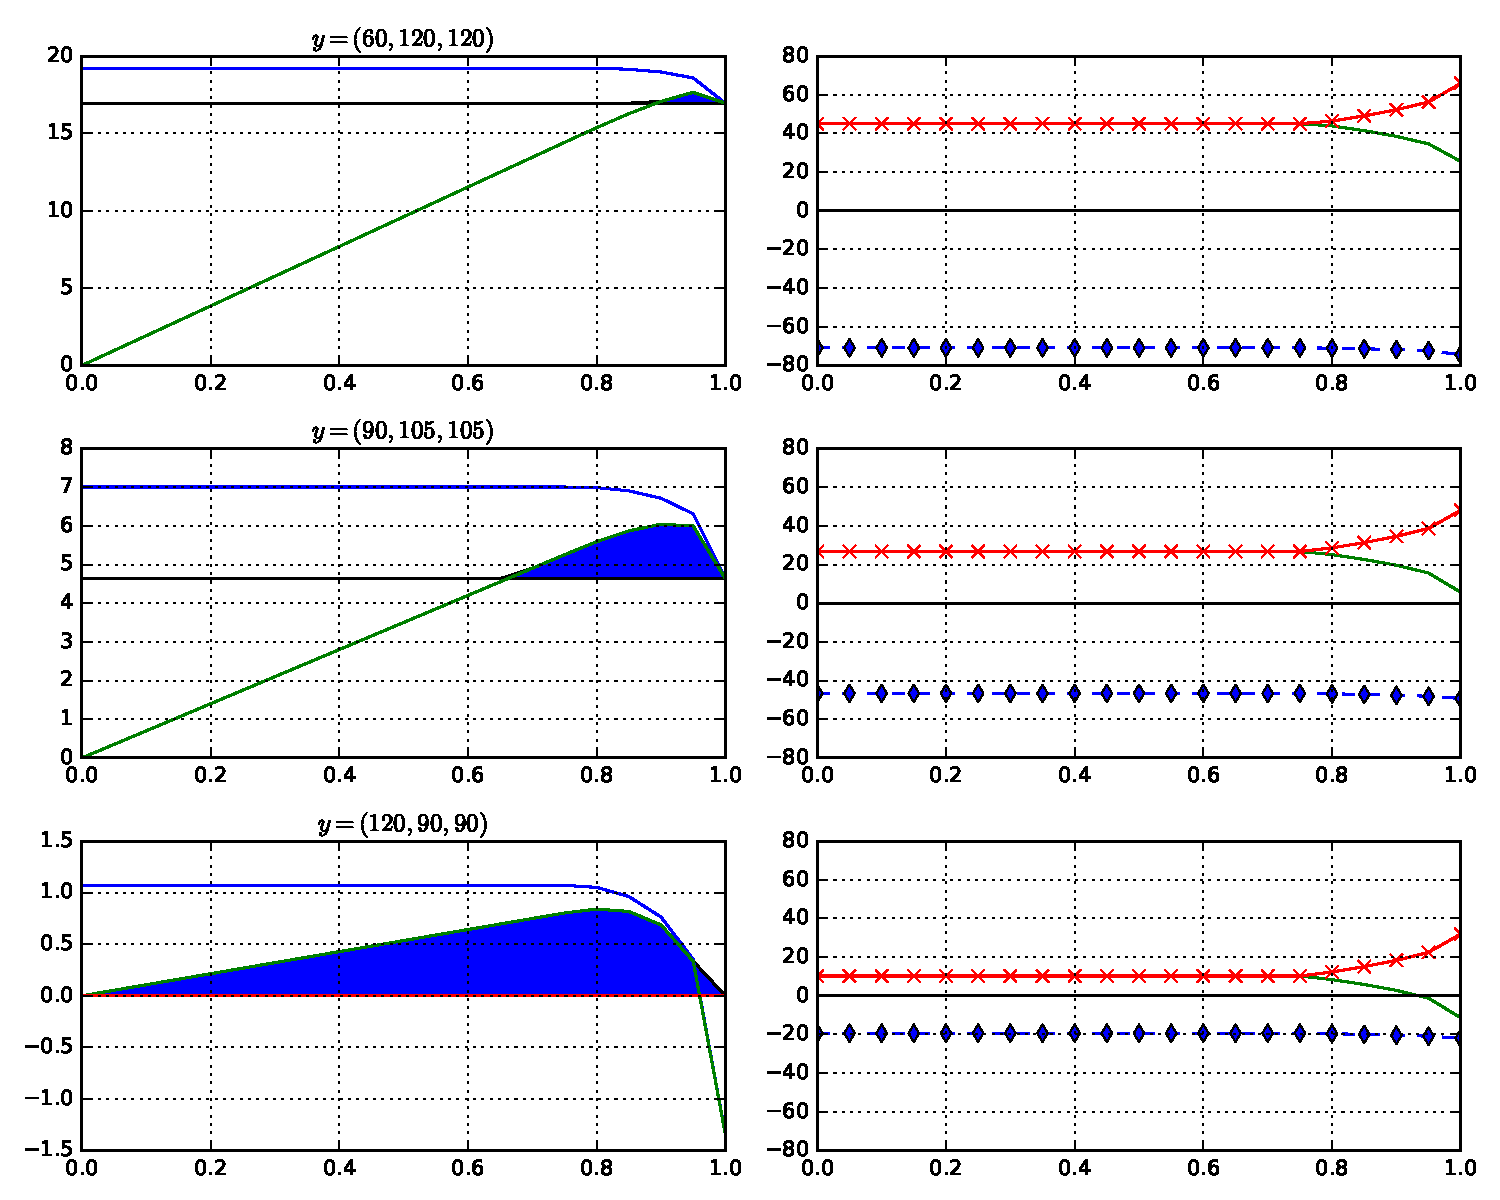
\includegraphics[width=1\textwidth]{fig_nonprofits.pdf}
\caption{\label{fig:nonprofit}Choice of non-profit status and initial endowment
income}
\end{figure}

In Figure \ref{fig:nonprofit} we illustrate the case where non-pecuniary
costs to breaking a promise not to renegotiate fall with $\alpha$
according to $\eta(\alpha)=10(1-\alpha)$ and hence that the overall
cost to renegotiation varies with $\alpha$ according to $\kappa(\alpha)=10(1-\alpha)/\alpha$.
The plots depict captured profits that would be achieved at different
levels $\alpha$ starting from three different initial endowment streams.
These three streams - (60, 120, 120), (90, 105, 105) and (120, 90,
90) \textendash{} are equal in their present value of 300 but differ
in terms of period 0 income (with remaining income allocated equally
across period 1 and 2). The higher of the two curved lines represents
`raw' profits $\Pi_{0}(C_{0}^{m\alpha};Y_{0})$ and the lower curve
captured profits $\alpha\Pi_{0}(C_{0}^{m\alpha};Y_{0})$. A horizontal
line has been drawn in to indicate the level of profits $\Pi_{0}(C_{0}^{mP};Y_{0})$
captured by a pure for-profit ($\alpha=1$). Consider the top panel
where the customer has initial income $(60,120,120)$. As this type
of customer wants to borrow heavily in period 0 profits to the bank
are large, even in the case of renegotiation-proof contracts. Adopting
non-profit status by lowering $\alpha$ confers limited profit gain
however: the cost of lowering alpha (giving up a share of already
high profits) is not compensated for by the gains from being able
to credibly commit to a smoother contract. However at $(90,105,105)$
the tradeoff is different and profits can be increased. In the picture
any non-profit with an $\alpha$ between approximately 0.7 and less
than one captures more profits than a pure for-profit. Finally for
customers with an endowment $(120,90,90)$ are already fairly close
to their preferred consumption stream so the profits to be captured
even under full commitment are not that large. Indeed in this case
a pure for-profit cannot earn positive profits. Here the cost of adopting
non-profit status is low compared to the gains, and we the simulation
reveal that any non-profit status firm captures more profits than
a pure for-profit, and maximum captured profits are achieved at around
$\alpha=0.7$.

We conclude this section with a note on the nature of profit-capture
restrictions faced by a nonprofit. Our assumption that the firm can
capture a fixed fraction of raw profits was useful for exposition
but is perhaps not realistic, and is not necessary for our results.
We might imagine that, at low levels of profits, the nonprofit can
capture most of the profits, and that as profits rise so do the restrictions
on the firm's ability to capture them. In other words, a nonprofit
captures $f\left(\Pi\right)$ of profits, where $f\left(0\right)=0$,
$0<f'\left(\Pi\right)<1$, and $f''\left(\Pi\right)<0.$ In such cases,
we can again clearly see how non-profit status could be attractive
to the firm: the concavity of $f$ can leave the enjoyment of profits
relatively unaffected while significantly loosening the no-renegotiation
constraint (since renegotiation would raise profits further, and since
$f$ is concave, these additional profits would count for little).

\subsection{Competition}

\subsubsection{Exclusive contracts}

Consider what would happen in the competitive market situation now
if contracts can be assumed to remain exclusive, so that any new surplus
in the event of a renegotiation between the bank and the period 1
self goes to the bank (this grants the bank monopoly power in period
1). A firm of type $\alpha$ will be led to offer contract terms to
solve 
\begin{align}
\underset{C_{0}}{max} & U_{0}\left(C_{0}\right)\nonumber \\
s.t. & \alpha\Pi_{0}(C_{0};Y_{0})\geq0\\
 & \Pi_{0}(C_{1}^{m1}(C_{1});C_{1})\leq\kappa(\alpha)
\end{align}

Here, as before, $\kappa(\alpha)=\frac{\eta(\alpha)}{\alpha}$, captures
the idea that the principals of a firm that adopts non-profit status
commit themselves to capturing a smaller share of raw profits and
may also suffer greater direct disutility from breaking promises to
customers. Let the contract that solves this program be denoted $C_{0}^{e\alpha}$
.

Consider first a field where all firms start as pure for-profits ($\alpha=1$).
If the no-renegotiation constraint binds, consumer welfare must be
lower than that when the firms can commit to not renegotiate since
an additional constraint is imposed. Starting from this situation
consider now one firm's strategic choice of whether to adopt non-profit
status (i.e. to change its ownership and governance structures to
an $\alpha=\bar{\alpha}<1$ relaxing the no-renegotiation constraint.
One firm deviating into nonprofit status in this way can make positive
profits. So, if the borrowers are sophisticated hyperbolics, in equilibrium
all firms become nonprofit. As proven in the appendix, competition
will ensure however that in equilibrium the principals of all firms
are capturing zero profits.

\subsubsection{Non-Exclusive Contracts}

In the previous section, we had a setting with competition in period
0 but exclusive contracting and monopoly power in period 1. Now, assume
that exclusivity and period 1 monopoly power disappears. Firms can
compete to renegotiate each other's contracts in period 1.

If there were only nonprofits in equilibrium, any one firm could make
positive profits by switching to for-profit status and undoing a rival
bank's contract in period 1. The advantages of undercutting other
firms' contracts outweigh the benefits of promising one's own clients
it will not renegotiate. As a result, equilibrium contracts will be
determined by for-profit firms, and consumers will be offered lower
commitment than from non-profit firms alone.\footnote{The same argument applies if banks can costlessly renegotiate other
bank's contracts.} Additionally, a smaller range of consumer types will be serviced
relative to the case with exclusive contracts.
\begin{prop}
Consider any $\bar{\alpha}<1$ and a corresponding $\eta\left(\bar{\alpha}\right)=\kappa$.

(a) In a competitive banking market with exclusive contracts, all
active firms will be nonprofits (contracts will be offered for $U_{0}^{A}\leq\bar{U}^{\alpha}$,
with $\bar{U}^{\alpha}$ as defined in Proposition 6).

(b) In a competitive banking market with non-exclusive contracts,
for-profits must exist in equilibrium (contracts will be offered for
$U_{0}^{A}\leq\bar{U}$, with $\bar{U}$ as defined in Proposition
2). 
\end{prop}

\section{Discussion and Extensions}

The model above formalizes the renegotiation problem faced by banks
that contract with hyperbolic discounters, and shows how the problem
is addressed in equilibrium contracts. Figure \ref{fig:Summary} summarizes
the key results of Sections 4-6. We show how contracts depend on relative
distances from the optimal autarky utility, $U_{0}^{F}$. The results,
taken together, generate some natural yet novel empirical predictions
that are in principle testable.

\begin{figure}
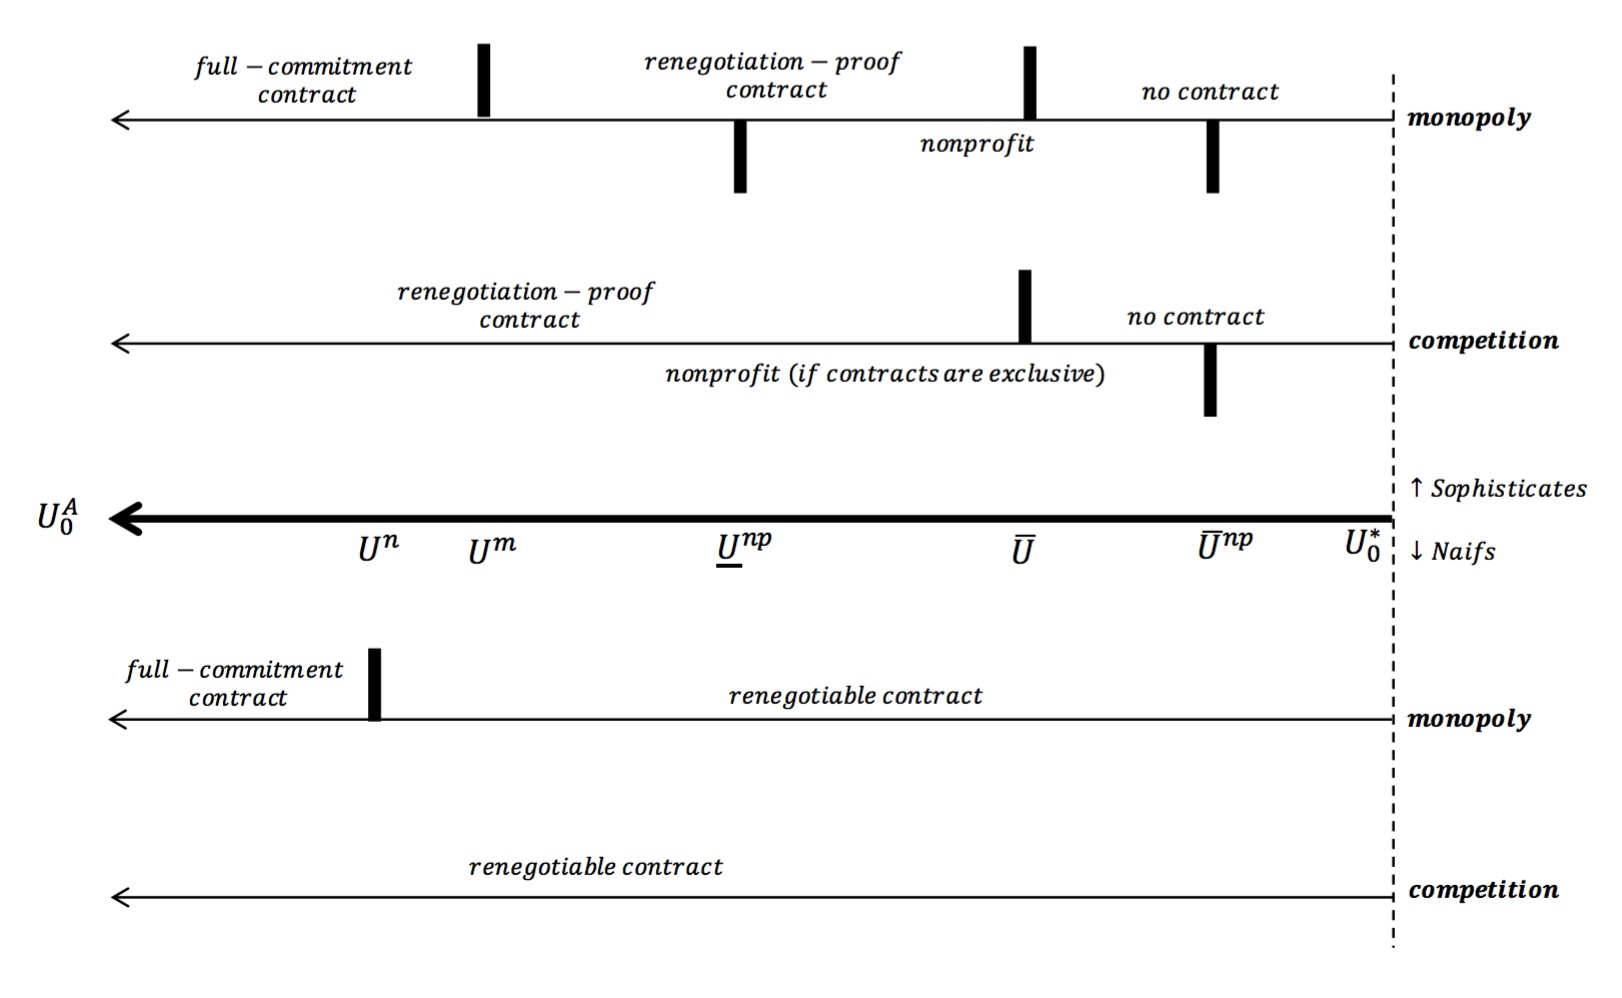
\includegraphics[scale=1.0]{fig_results}

\caption{\label{fig:Summary}Summary of results}
\end{figure}

We first discuss naive hyperbolic discounters. Under monopoly, contracts
will be subject to renegotiation if the consumer is close enough to
optimal autarky; if not, the full-commitment contract leaves the consumer
with so little consumption that there is no point renegotiating. The
parameter region in which contracts are renegotiated is relatively
large, and even includes cases where the sophisticate would be offered
a full-commitment contract. The renegotiable contract involves less
period-0 consumption that the full-commitment contract as this allows
the bank to exploit renegotiation possibilities most comprehensively.

Under competition, any contract will be renegotiated, even for consumers
whose autarky outcomes are very poor. This is because competitive
full-commitment contracts always leave consumers with relatively high
levels of future consumption. The implications for contract terms
are ambiguous.

Next, we turn to sophisticated hyperbolic discounters under monopoly.
If the consumer's smoothing needs are large (i.e. autarky utility
is low), full-commitment is feasible since the contract terms leave
little that is susceptible to renegotiation. If smoothing needs are
moderate, the consumer is offered a renegotiation-proof contract which
has a larger period-0 consumption than the full-commitment contract
(this serves to reduce the contract's susceptibility to renegotiation).
If smoothing needs are small, the consumer is better off in autarky
than in any contract that satisfies the renegotiation-proof constraint.
As a result of the problem of renegotiation, such consumers will not
be offered contracts.

Under competition, sophisticates will not be offered full-commitment
contracts. Since full-commitment would entail high consumption levels
in periods 1 and 2 regardless of autarky utility, the renegotiation-proofness
constraint must always bind. As under naivete, the implications for
contract terms are ambiguous.

Finally, we derive conditions under which banks will operate as nonprofits.
A monopoly will switch to a nonprofit if, as a for-profit its profits
were close to zero (above or below). In these cases, the bank is willing
to forgo some enjoyment of its profits in exchange for a loosened
renegotiation-proofness constraint. So, nonprofits will be able to
serve some consumers relatively closer to optimal autarky utility,
ones who would be unbanked under for-profit monopoly.

Under competition, banks should operate as nonprofits if contracts
are exclusive, as they can capture the surplus from improved contracts
possible under nonprofit status. If contracts are non-exclusive, no
bank can benefit from operating as a nonprofit, and for-profit banks
prevail.

\subsection{Additional Considerations}

Our model delivers predictions about how renegotiation concerns affect
commitment contracts, and about parameter regions in which these concerns
actually matter. In particular, we generate comparative statics over
autarky utilities. Autarky utility is not informative in isolation,
but in conjunction with total income serves as an indicator of the
extent of smoothing that remains to be provided by a bank. As we show,
contract terms depend in particular ways at different degrees of smoothing
needs.

The sizes of relevant parameter regions discussed above will vary
according to other parameter values such as the cost of renegotiation,
$\kappa$, and total income, $y$. For example, as $\kappa$ rises
there will be an expansion of the parameter region in which full commitment
survives. On the other hand, as $y$ rises, commitment in general
will be harder to sustain since contracts terms must allow for higher
consumption in periods 1 and 2.

While the focus of our paper is on contracts, a few observations on
welfare can be made. Under hyperbolic discounting, there is no obvious
notion of welfare, and for our purpose we take it to the discounted
utility of the Zero-self. Clearly, for sophisticated hyperbolic discounters
under monopoly, welfare remains constant regardless of renegotiation
concerns and bank governance\textendash the consumer is always left
with autarky utility. Under competition, welfare is lower under renegotiation-proof
contracts relative to full-commitment (when the constraint binds),
and nonprofits serve to raise welfare.

\subsubsection{Equilibria allowing period 1 contracts}

Our preceding analysis made the simplifying assumption that contracts
between consumers and banks could only be initiated in period 0. The
alternative to a period 0 contract was autarky for the consumer in
the monopoly case and zero profits for the bank under competition.
This served to streamline the analysis. We now discuss the interesting
problem of how the contract space is enriched by allowing unbanked
consumers to sign two-period contracts in period 1, possibly without
contracting in period 0.\footnote{We thank Abhijit Banerjee for very helpful discussions about this
point.} The main change will relate to the formulation of reservation values
and their implications for the shape and feasibility of the period
0 contracts. The main qualitative results of the paper go through
but the discussion raises interesting questions about circumstances
where consumers could be better off under an autarky economy compared
to one with a financial intermediary.

Consider the monopolist bank facing a sophisticated hyperbolic discounter.
If a contract were not signed in period 0, they would meet again in
period 1. In period 1, the contract must satisfy the One-self's participation
constraint, which would be determined by some unbanked consumption
path $C_{1}^{A'}$. This can be stated formally. Given some consumption
path $C_{1}^{A'}$, the bank solves: 
\begin{align*}
\underset{C_{1}}{\max}\text{ }{\Pi_{1}\left(C_{1};C_{1}^{A'}\right)}\\
\text{s.t. }U_{1}\left(C_{1}\right)\geq U_{1}\left(C_{1}^{A'}\right)
\end{align*}

Let the solution be denoted $C_{1}^{m'}$. Two observations can be
made. First, the bank can always offer a period 1 contract that delivers
nonnegative profits. This is because any contract will satisfy One-self's
optimality condition, $u'\left(c_{1}^{m'}\right)=\beta u'\left(c_{2}^{m'}\right)$.
So, except in the special case where the autarky consumption path
satisfies this condition, the bank can make positive profits in period
1. Second, the autarky consumption path $C_{1}^{A'}$ might differ
from $C_{1}^{A}$, the consumer's autarky utility in the absence of
banking. In other words, $C_{1}^{A}$ maximizes $U_{0}\left(C_{0}^{A}\right)$
while $C_{1}^{A'}$ maximizes $U_{0}\left(c_{0}^{A'},c_{1}^{m'},c_{2}^{m'}\right)$.
In the latter case, period 0 anticipates that consumption across periods
1 and 2 is guaranteed to satisfy period 1's optimality condition.
We can denote $C_{0}^{B}\equiv\left(c_{0}^{A'},c_{1}^{m'},c_{2}^{m'}\right)$,
which corresponds to a Zero-self utility of $U_{0}^{B}$.

In period 0, any contract must meet the Zero-self's reservation utility,
$U_{0}^{B}$: 
\begin{align*}
\underset{C_{0}}{max} & \Pi_{0}\left(C_{0};Y_{0}\right)\\
\text{s.t.} & \text{\ensuremath{U_{0}\left(C_{0}\right)\geq U_{0}^{B}}}
\end{align*}

The maximization problem looks familiar, apart from the modified reservation
utility. The Zero-self's discounted utility from such a contract is
no longer monotonic in her Zero-self's full-autarky utility, $U_{0}^{A}$.
For example, consider two hypothetical consumers who in autarky must
consume their income streams, which deliver the same autarky utility
but through different consumption paths: consumer X has $c_{1}^{A}=c_{2}^{A}$
while consumer Y has $c_{1}^{A}>c_{2}^{A}$ in a way that satisfies
period 1's optimality condition. Then, for consumer X, $U_{0}^{B}<U_{0}^{A}$
while for consumer Y, $U_{0}^{B}=U_{0}^{A}$. It follows that, since
period 0 contracts depend on the distribution of future consumption,
a consumer who fares relatively better in the absence of a bank may
fare relatively worse under a banking contract.

Given this benchmark full-commitment contract, the renegotiation-proof
contract can be solved for by adding a no-renegotiation constraint
to the above maximization problem. The constraint is the same as used
previously, and again narrows the set of contracts that can be offered
in period 0. As in Proposition 2 (parts a and c), the renegotiation-proof
constraint results in lower profits and greater period 0 consumption
relative to full-commitment. These results are independent of the
period 0 reservation utility and therefore remain unchanged.

A key difference here, however, is that a renegotiation-proof contract
will be offered to all consumers (unlike before, where the bank was
better off not contracting with consumers whose autarky utility left
them close enough to the first-best). Intuitively, this is because
the alternative to a period 0 contract is not autarky; rather, it
is a period 1 contract that tilts consumption in period 1's favor.
Since, in period 0, the bank can at least offer the consumer a consumption
path of $C_{0}^{B}$, it ensures that a contract will be accepted.

By opening up the possibility of period 1 contracts, we introduce
an additional consideration\textendash the same bank that offers commitment
itself creates a need for commitment. By threatening to fully indulge
the One-self's preferences, the bank is always able to induce the
Zero-self to accept an offer of partial commitment, no matter how
weak.

Finally, observe that the bank's decision about whether to operate
as a nonprofit is subject to the same tradeoff between improved commitment
and reduced enjoyment of profits. However, the attractiveness of nonprofit
status drops (relative to the case where period 1 contracts are disallowed)
due to the fact that even the for-profit bank finds it profitable
to offer contracts to consumers at all levels of autarky utility.

Next, we turn to competition. In most cases, the possibility of period
1 contracts leaves our previous analysis unaltered. This is because
competitive contracts do not depend on autarky utility. The only modification
to our previous results relates to Proposition 3 (part b). Now, the
consumer will accept a period 0 renegotiation-proof contract at any
autarky utility since not doing so exposes her to a period 1 contract
that fully satisfies period 1's taste for imbalanced consumption. 

\section{Conclusion}

The starting point for this paper is the observation that the solution
to any commitment problem must also address a renegotiation problem.
We show how the renegotiation problem affects different types of consumers
and how it changes contract terms in sometimes unexpected ways. In
this context, we also provide a rationalization of commercial nonprofits
in the absence of asymmetric information.

We argue that the model sheds some light on trends in microfinance,
payday lending, and mortgage lending. We hope this paper also offers
a framework that can be built upon. The incorporation of additional
`real-world' factors could improve our understanding of particular
institutions and generate empirically relevant comparative statics.
Examples of these include nondeterministic incomes, private and heterogenous
types, collateral and strategic default, and longer time horizons.

Finally, the differences between monopoly and competition open up
some new, potentially interesting questions. How does market structure
evolve and what are the implications for commitment? And through this
evolution might there emerge third parties to contracts between consumers
and banks that can more effectively enforce the commitment that is
sought after on both sides of the market?


\section{Appendix: CRRA Derivations and Proofs}

\subsection{Full-commitment}

\subsubsection{Competition}

The first-order conditions are:

\begin{equation}
c_{1}=\beta{}^{\frac{1}{\rho}}c_{0}\label{eq:FOCc0c1}
\end{equation}

\begin{equation}
c_{2}=c_{1}\label{eq:FOCc1c2}
\end{equation}

The first-order conditions and budget constraint can be combined to
give:
\begin{equation}
c_{1}=\frac{y-c_{0}}{2}\label{eq:budgetplus}
\end{equation}

Then, the competitive full commitment contract $C_{0}^{F}$ is:

\begin{align}
c_{0}^{F} & =\frac{y}{1+2\beta^{\frac{1}{\rho}}}\label{eq:CF}\\
c_{1}^{F} & =c_{2}^{F}=\beta^{\frac{1}{\rho}}c_{0}^{F}\label{eq:CF1}
\end{align}
or compactly on a single line:

\begin{equation}
C_{0}^{F}=\left(1,\beta^{\frac{1}{\rho}},\beta^{\frac{1}{\rho}\right)\cdot\left(\frac{y}{1+2\beta^{\frac{1}{\rho}}}\right) \end{equation}

\subsubsection{Monopoly}

For the monopolist bank that offers full-commitment, the solution
is determined by the first-order condition and the consumer's participation
constraint to yield: 
\begin{align}
C_{0}^{mF} & =\left(1,\beta^{\frac{1}{\rho}},\beta^{\frac{1}{\rho}}\right)\cdot\left(\frac{U_{0}^{A}\left(1-\rho\right)}{1+2\beta^{\frac{1}{\rho}}}\right)^{\frac{1}{1-\rho}}\label{eq:c-mf}\\
\Pi_{0}\left(C_{0}^{mF};Y_{0}\right) & =y-\left(U_{0}^{A}\left(1-\rho\right)\right)^{\frac{1}{1-\rho}}\left(1+2\beta^{\frac{1}{\rho}}\right)^{\frac{-\rho}{1-\rho}}\label{eq:pi-mf}
\end{align}

\subsection{Renegotiation}

\subsubsection{Renegotiated contracts}

Given an existing continuation contract $C_{1}^{0}$, assuming the
contract is renegotiated, the competitively renegotiated contract
will be: 
\begin{equation}
C_{1}^{1}\left(C_{1}^{0}\right)=\left(1,\beta^{\frac{1}{\rho}}\right)\cdot\left(\frac{c_{1}^{0}+c_{2}^{0}-\kappa}{1+\beta^{\frac{1}{\rho}}}\right)\label{eq:c-r}
\end{equation}

And under monopoly, the renegotiated contract will be:
\begin{equation}
C_{1}^{m1}\left(C_{1}^{0}\right)=\left(1,\beta^{\frac{1}{\rho}}\right)\cdot\left(\frac{(c_{1}^{0})^{1-\rho}+\beta(c_{2}^{0})^{1-\rho}}{1+\beta^{\frac{1}{\rho}}}\right)^{\frac{1}{1-\rho}}\label{eq:m-r}
\end{equation}

The corresponding profit gains from renegotiation in the monopoly
case are: 
\begin{equation}
\Pi_{1}\left(C_{1}^{m1}\left(C_{1}^{0}\right);C_{1}^{0}\right)=\left(c_{1}^{0}+c_{2}^{0}\right)-\left((c_{1}^{0})^{1-\rho}+\beta(c_{2}^{0})^{1-\rho}\right)^{\frac{1}{1-\rho}}\left(1+\beta^{\frac{1}{\rho}}\right)^{\frac{-\rho}{1-\rho}}\label{eq:pi-r}
\end{equation}


\subsubsection{No-renegotiation constraint}

Conditions \ref{eq:no-reg-comp} and \ref{eq:no-reg-monop} are equivalent to writing: 
$$u(c_1^0)+\beta u(c_2^0) \ge u(c_1^1)+\beta u(c_2^1) $$
$$ c_1^1+c_2^1-\kappa \ge  c_1^0+c_2^0 $$
In this CRRA case the second condition can be rewritten
$$c_1^1 \ge \frac{c_1^0+c_2^0-\kappa}{1+\beta^\frac{1}{\rho}}$$
Substituting this into the first
yields
the following no-renegotiation condition which will be identical in the period 1 monopoly and competitive case:

$$u(c_1^0)+\beta u(c_2^0)\ge ({1+\beta^\frac{1}{\rho}})u \left ( \frac{c_1^0+c_2^0-\kappa}{1+\beta^\frac{1}{\rho}}
\right ) $$
Alternatively, this condition can be written:
\begin{equation}
\left(c_{1}^{0}+c_{2}^{0}\right)-\left((c_{1}^{0})^{1-\rho}+\beta(c_{2}^{0})^{1-\rho}\right)^{\frac{1}{1-\rho}}\left(1+\beta^{\frac{1}{\rho}}\right)^{\frac{-\rho}{1-\rho}}\leq\kappa\label{eq:no-renegotiation}
\end{equation}

\textendash{} \textendash{} \textendash{} \textendash{} \textendash{}
\textendash{} \textendash{} \textendash{} 

\subsection{Renegotiation}

In both cases we are assuming that $\kappa$ is not large enought
to eliminate the gains to trade. 

An alternate way to restate the above is the following: Let $s$ and
$\alpha$ be defined such that $c_{1}=\alpha s$ and $c_{2}=\left(1-\alpha\right)s$.
Then: 
\begin{equation}
C_{1}^{m1}\left(C_{1}^{0}\right)=\left(s,s\beta^{\frac{1}{\rho}}\right)\cdot\left(\frac{\alpha^{1-\rho}+\beta\left(1-\alpha\right)^{1-\rho}}{1+\beta^{\frac{1}{\rho}}}\right)^{\frac{1}{1-\rho}}\label{eq:c-r-alpha}
\end{equation}

Profit gains from renegotiation become: 
\begin{equation}
\Pi_{1}\left(C_{1}^{m1}\left(C_{1}\right);C_{1}\right)=\left(s\right)\left(1-\left(\alpha^{1-\rho}+\beta\left(1-\alpha\right)^{1-\rho}\right)^{\frac{1}{1-\rho}}\right)\label{eq:renegotiation-profits}
\end{equation}

By construction, profits from renegotiation are strictly positive
(and increasing in $s$), except in the special case where $C_{1}$
is optimal from period 1's perspective ($\left(1-\alpha\right)=\beta^{\frac{1}{\rho}}\alpha$),
in which case they are $0$. It can also easily be confirmed that
profits from renegotiation fall in $\alpha$ as long as the allocation
is such that period 1 would like a larger $\alpha$ than the current
contract offers.

\textbf{\textit{Proof of Proposition 1:}} (a) In any full-commitment
contract, $\alpha=\frac{1}{2}$. Inserting this into (\ref{eq:renegotiation-profits}),
the following must be satisfied for a full-commitment contract to
survive: 
\begin{equation}
k\geq s\left(1-\frac{1}{2}\left(1+\beta\right)^{\frac{1}{1-\rho}}\left(1+\beta^{\frac{1}{\rho}}\right)^{\frac{-\rho}{1-\rho}}\right)\label{eq:max-kappa-part}
\end{equation}
Substituting for $s=y-c_{0}^{F}$ from the competitive full-commitment
contract, we can rewrite the above condition as: 
\begin{equation}
k\geq\frac{2\beta^{\frac{1}{\rho}}y}{1+2\beta^{\frac{1}{\rho}}}\left(1-\frac{1}{2}\left(1-\beta\right)^{\frac{1}{1-\rho}}\left(1+\beta^{\frac{1}{\rho}}\right)^{\frac{-\rho}{1-\rho}}\right)\equiv\bar{\kappa}\label{eq:max-kappa}
\end{equation}
Since in any full-commitment contract (monopoly and competition),
$s$ will be no larger than $\frac{2\beta^{\frac{1}{\rho}}y}{1+2\beta^{\frac{1}{\rho}}}$,
no full-commitment contract will be renegotiated if $\kappa\geq\bar{\kappa}$.

(c) If $\kappa<\bar{\kappa}$, condition \ref{eq:max-kappa} fails,
so the competitive full-commitment contract cannot survive.

(b) The monopolist full-commitment contract will not survive if $s$
is sufficiently large. Since $s^{mF}$ is exponentially (and therefore
monotonically) increasing in $U_{0}^{A}$, there must be some $U^{m}$
such that the contract will not survive if and only if $U_{0}^{A}>U^{m}$.
Since the contract cannot survive at $U_{0}^{F}$ (here, the contract
is identical to the competitive contract), $U^{m}<U_{0}^{F}$. $\Square$

\subsection{Renegotiation-Proof Contracts}

\subsubsection{Sophisticated Hyperbolic Discounters}

When the renegotiation-proofness constraint binds, consumption in
periods 1 and 2 must satisfy: 
\begin{equation}
\left(s\right)\left(1-\left(\alpha^{1-\rho}-\beta\left(1-\alpha\right)^{1-\rho}\right)^{\frac{1}{1-\rho}}\left(1+\beta^{\frac{1}{\rho}}\right)^{\frac{-\rho}{1-\rho}}\right)=\kappa\label{eq:rp-constraint}
\end{equation}

For any $s$, there may be two values of $\alpha$ that satisfy the
constraint with equality\textendash one with too little consumption
relative to period 1's optimal, one with too much consumption relative
to period 1's optimal. The relevant value for us is the first. This
defines a continuous function $\alpha\left(s\right)$. 
\begin{equation}
\alpha\left(s\right)=min\left\{ \alpha:\left(s\right)\left(1-\left(\alpha^{1-\rho}+\beta\left(1-\alpha\right)^{1-\rho}\right)^{\frac{1}{1-\rho}}\left(1+\beta^{\frac{1}{\rho}}\right)^{\frac{-\rho}{1-\rho}}\right)=\kappa\right\} \label{eq:alpha}
\end{equation}

As $s$ rises, to continue satisfying the constraint we must have
$\alpha\left(s\right)$ rising too (if fractions stayed constant,
profits from renegotiation would rise).

We can also rewrite the first-order condition of the bank's maximization
problem using the new notation. For any $s$ and $\alpha$, let $V\left(s,\alpha\right)=u\left(\alpha s\right)+u\left(\left(1-\alpha\right)s\right)$.
This is the discounted utility over periods 1 and 2, from period 0's
perspective. The solution, $C_{0}=$$\left(c_{0},\alpha s,\left(1-\alpha\right)s\right)$,
must satisfy: 
\begin{equation}
\frac{du\left(c_{0}\right)}{dc_{0}}=\beta\frac{dV\left(s,\alpha\right)}{ds}\label{eq:du-dv}
\end{equation}

In other words, at the profit-maximizing contract the marginal dollar
should be equally valuable whether consumed immediately or distributed
across future periods.

\textbf{\textit{Proof of Proposition 2:}} (a) Since the full-commitment
profit-maximizing contract was uniquely determined, and since it does
not satisfy the renegotiation-proofness constraint, the renegotiation-proof
contract must yield lower profits than the full-commitment contract
does.

(b) Clearly, $\Pi_{0}\left(C_{0}^{mP};Y_{0}\right)$ falls strictly
in $U_{0}^{A}$ (if autarky utility falls, the bank can always do
better, at least by simply lowering $c_{0}$). Since at $U_{0}^{A}=U^{m}$,
$\Pi_{0}\left(C_{0}^{mP};Y_{0}\right)=\Pi_{0}\left(C_{0}^{mF};Y_{0}\right)>0$
and at $U_{0}^{A}=U_{0}^{F}$, $\Pi_{0}\left(C_{0}^{mP};Y_{0}\right)<\Pi_{0}\left(C_{0}^{mF};Y_{0}\right)=0$,
there must be some intermediate autarky utility above which the bank's
maximized profits will be negative.

(c) consider any $c_{0}\leq c_{0}^{mF}$ and $s$ such that $U_{0}\left(c_{0},\frac{s}{2},\frac{s}{2}\right)=U_{0}^{A}$.
We can find the corresponding $\bar{s}$ that, while satisfying the
participation constraint, gives the same utility from period 0's perspective:

\begin{align}
V\left(s,\frac{1}{2}\right) & =\bar{V}\left(\bar{s},\alpha\left(\bar{s}\right)\right)\label{eq:v=00003D00003D00003Dvbar1}\\
\Rightarrow2\frac{\left(\frac{1}{2}s\right)^{1-\rho}}{1-\rho} & =\frac{\left(\alpha\left(\bar{s}\right)\bar{s}\right)^{1-\rho}}{1-\rho}+\frac{\left(\left(1-\alpha\left(\bar{s}\right)\right)\bar{s}\right)^{1-\rho}}{1-\rho}\label{eq:v-vbar2}\\
\Rightarrow\bar{s} & =s\left(\frac{2\left(\frac{1}{2}\right)^{1-\rho}}{\alpha\left(\bar{s}\right)^{1-\rho}+\left(1-\alpha\left(\bar{s}\right)\right)^{1-\rho}}\right)^{\frac{1}{1-\rho}}\label{eq:v-vbar3}
\end{align}

From this, we get the following inequality: 
\begin{align}
\frac{dV\left(\bar{s},\alpha\left(\bar{s}\right)\right)}{ds} & =\bar{s}^{-\rho}\left(\alpha\left(\bar{s}\right)^{1-\rho}+\left(1-\alpha\left(s\right)\right)^{1-\rho}\right)+\frac{d\alpha\left(\bar{s}\right)}{ds}\bar{s}^{1-\rho}\left(\alpha\left(\bar{s}\right)^{-\rho}-\left(1-\alpha\right)^{-\rho}\right)\label{eq:dv-ds1}\\
 & <\bar{s}^{-\rho}\left(\alpha\left(\bar{s}\right)^{1-\rho}+\left(1-\alpha\left(s\right)\right)^{1-\rho}\right)\label{eq:dv-ds2}\\
 & =s^{-\rho}\left(2\left(\frac{1}{2}\right)^{1-\rho}\right)\left(\frac{2\left(\frac{1}{2}\right)^{1-\rho}}{\alpha\left(\bar{s}\right)^{1-\rho}+\left(1-\alpha\left(\bar{s}\right)\right)^{1-\rho}}\right)^{\frac{-1}{1-\rho}}\label{eq:dv-ds3}\\
 & <s^{-\rho}\left(2\left(\frac{1}{2}\right)^{1-\rho}\right)=\frac{dV\left(s,\frac{1}{2}\right)}{ds}\label{eq:dv-ds4}
\end{align}

The first line above splits the effect of $s$ on $V$ into two\textendash the
first term represents the change in utility holding $\alpha$ constant,
and the second term represents the (negative) effect of the further
skewing of consumption that results from a rise in $s$. The final
inequality follows from the fact that, since $\bar{s}>s^{mF}$, the
renegotiation constraint must bind so that $\alpha\left(\bar{s}\right)>\frac{1}{2}$.
Finally, the following inequality holds: 
\begin{align}
\frac{du\left(c_{0}\right)}{dc_{0}} & \geq\frac{du\left(c_{0}^{mF}\right)}{dc_{0}}=\beta\frac{dV\left(s^{mF},\frac{1}{2}\right)}{ds}\label{eq:dudc-dvds1}\\
 & \geq\beta\frac{dV\left(s,\frac{1}{2}\right)}{ds}>\beta\frac{dV\left(\bar{s},\alpha\left(\bar{s}\right)\right)}{ds}\label{eq:dudc-dvds2}
\end{align}

We have shown that at any $c_{0}\leq c_{0}^{mF}$, for a contract
that satisfies the renegotiation-proofness constraint, the marginal
utility of period 0 consumption will be higher than the discounted
marginal utility of future consumption, so the bank could earn strictly
higher profits by raising $c_{0}$ and lowering $s$ further. Therefore,
in the renegotiation-proof contract, $c_{0}^{mP}>c_{0}^{mF}$. $\Square$

\textbf{\emph{Proof of Proposition 3:}} (a) We know that $U_{0}\left(C_{0}^{F}\right)=U_{0}^{F}$.
By assumption, since the renegotiation-proofness constraint is binding,
the renegotiation-proof contract cannot offer the optimal consumption
path. Therefore $U_{0}\left(C_{0}^{P}\right)<U_{0}\left(C_{0}^{F}\right)$.

(b) Consider $\bar{U}$, as constructed in Proposition 2. If $U_{0}^{A}>\bar{U}$,
it is impossible to construct a contract that earns nonnegative profits
and gives the consumer at least autarky utility. Therefore, any contract
that earns zero profits would give the period 0 consumer less than
autarky utility. (As an aside, observe that $\bar{U}=U_{0}\left(C_{0}^{P}\right)$.)

(c) At the full-commitment contract: 
\begin{equation}
\frac{du\left(c_{0}^{F}\right)}{dc}=\beta\frac{dV\left(s^{F},\frac{1}{2}\right)}{ds}=\left(s^{F}\right)^{-\rho}\left(2\left(\frac{1}{2}\right)^{1-\rho}\right)
\end{equation}
Consider a renegotiation-proof contract with $c_{0}=c_{0}^{F}$. To
keep bank profits zero, this contract would also have $s=s^{F}$.
But in the renegotiation-proof contract, $s$ must be divided according
to the fraction $\alpha\left(s^{F}\right)$. So: 
\begin{align}
\frac{dV\left(s^{F},\alpha\left(s^{F}\right)\right)}{ds} & =\left(s^{F}\right)^{-\rho}\left(\alpha\left(s^{F}\right)^{1-\rho}+\left(1-\alpha\left(s^{F}\right)\right)^{1-\rho}\right)\nonumber \\
 & +\frac{d\alpha\left(s^{F}\right)}{ds}\left(s^{F}\right)^{1-\rho}\left(\alpha\left(s^{F}\right)^{-\rho}-\left(1-\alpha\left(s^{F}\right)\right)^{-\rho}\right)\label{eq:dv-ds-comp}
\end{align}
The first term\textendash the direct effect of a change in $s$\textendash is
weakly less than $\frac{dV\left(s^{F},\frac{1}{2}\right)}{ds}$ if
$\rho\leq1$ and strictly greater if $\rho>1$. The second term\textendash the
component of $\frac{dV}{ds}$ that is driven by the change in $\alpha$\textendash is
strictly negative. Therefore, if $\rho<1$, $\frac{dV\left(s^{F},\alpha\left(s^{F}\right)\right)}{ds}<\frac{dV\left(s^{F},\frac{1}{2}\right)}{ds}=\frac{du\left(c_{0}^{F}\right)}{dc}$,
so the renegotiation-proof contract must satisfy $c_{0}^{P}>c_{0}^{F}$.

Next, we consider the case when $\rho>1$. We can make the following
observations about $\alpha\left(s\right)$. First, $\underset{\kappa\rightarrow0}{lim}\alpha\left(s\right)=\frac{\beta^{\frac{-1}{\rho}}}{1+\beta^{\frac{-1}{\rho}}}$
(this follows from the fact that at $\kappa=0$, the contract must
satisfy $u'\left(c_{1}\right)=\beta u'\left(c_{2}\right)$). Second,
implicitly differentiating equation \ref{eq:alpha} with respect to
$s$, and combining it with the previous limit result, we get $\underset{\kappa\rightarrow0}{lim}\frac{d\alpha\left(s\right)}{ds}=0$.
Therefore, if $\rho>1$ and $\kappa$ is small enough, the second
term in Equation \ref{eq:dv-ds-comp} will be sufficiently small in
magnitude that $\frac{dV\left(s^{F},\alpha\left(s^{F}\right)\right)}{ds}>\frac{dV\left(s^{F},\frac{1}{2}\right)}{ds}=\frac{du\left(c_{0}^{F}\right)}{dc}$.
In this case, the renegotiation-proof contract must satisfy $c_{0}^{P}<c_{0}^{F}$.
$\Square$

If $\kappa=0$, the renegotiation-proof contracts can be explicitly
derived since in any contract it must be true that $c_{2}=\beta^{\frac{1}{\rho}}c_{1}$.
Solving the respective maximization problems, we get the following
equilibrium contracts for monopoly and competition, respectively:
\begin{align}
C_{0}^{mP}= & \left(\left(\frac{U_{0}^{A}\left(1-\rho\right)}{1+\beta^{\frac{1}{\rho}}\left(\frac{\left(1+\beta^{\frac{1-\rho}{\rho}}\right)^{\frac{1}{\rho}}}{\left(1+\beta^{\frac{1}{\rho}}\right)^{\frac{1-\rho}{\rho}}}\right)}\right)^{\frac{1}{1-\rho}},\left(\frac{\beta+\beta^{\frac{1}{\rho}}}{1+\beta^{\frac{1}{\rho}}}\right)^{\frac{1}{\rho}}c_{0}^{mP},\beta^{\frac{1}{\rho}}\left(\frac{\beta+\beta^{\frac{1}{\rho}}}{1+\beta^{\frac{1}{\rho}}}\right)^{\frac{1}{\rho}}c_{0}^{mP}\right)\label{eq:zerokappa-monop}\\
C_{0}^{P}= & \left(\frac{y}{1+\beta+\beta^{\frac{1}{\rho}}},\left(\frac{\beta+\beta^{\frac{1}{\rho}}}{1+\beta^{\frac{1}{\rho}}}\right)c_{0}^{P},\beta^{\frac{1}{\rho}}\left(\frac{\beta+\beta^{\frac{1}{\rho}}}{1+\beta^{\frac{1}{\rho}}}\right)c_{0}^{P}\right)\label{eq:zerokappa-comp}
\end{align}

It can easily be established that $c_{0}^{mP}>c_{0}^{mF}$, $c_{0}^{P}>c_{0}^{mF}$
if $\rho>1$, and $c_{0}^{P}<c_{0}^{mF}$ if $\rho<1$.

\subsubsection{Naive Hyperbolic Discounters}

Suppose the monopolist intends to renegotiate the contract. The maximization
problem, combined with the expression for $C_{1}^{m1}\left(C_{1}\right)$
(\ref{eq:c-r-alpha}), simplifies to:

\begin{align}
\underset{c_{0},c_{1},c_{2}}{max} & y-c_{0}-\frac{\left(c_{1}^{1-\rho}+\beta c_{2}^{1-\rho}\right)^{\frac{1}{1-\rho}}}{\left(1+\beta^{\frac{1}{\rho}}\right)^{\frac{\rho}{1-\rho}}}-\kappa\\
s.t. & \frac{c_{0}^{1-\rho}}{1-\rho}+\beta\frac{c_{1}^{1-\rho}}{1-\rho}+\beta\frac{c_{2}^{1-\rho}}{1-\rho}\geq U_{0}^{A}
\end{align}

The partial derivatives of the resulting Lagrangian are: 
\begin{align}
\frac{\partial\mathcal{L}}{\partial c_{0}} & =-1-\lambda c_{0}^{-\rho}\label{eq:L0}\\
\frac{\partial\mathcal{L}}{\partial c_{1}} & =c_{1}^{-\rho}\left[-\left(\frac{c_{1}^{1-\rho}+\beta c_{2}^{1-\rho}}{1+\beta^{\frac{1}{\rho}}}\right)^{\frac{\rho}{1-\rho}}-\lambda\beta\right]\label{eq:L1}\\
\frac{\partial\mathcal{L}}{\partial c_{2}} & =c_{2}^{-\rho}\left[-\beta\left(\frac{c_{1}^{1-\rho}+\beta c_{2}^{1-\rho}}{1+\beta^{\frac{1}{\rho}}}\right)^{\frac{\rho}{1-\rho}}-\lambda\beta\right]\label{eq:L2}
\end{align}

An interior solution, with $\frac{\partial\mathcal{L}}{\partial c_{1}}=0$
and $\frac{\partial\mathcal{L}}{\partial c_{2}}=0$ does not exist
(on a $c_{1}-c_{2}$ plot, the two first-order conditions do not intersect).
If $\rho<1$, the Lagrangian is maximized at a corner solution with
$c_{1}=0$. If $\rho>1$, the Lagrangian is maximized at the limit
as $c_{2}$ approaches infinity. Using this, the maximization problem
can be re-solved. If $\rho<1$: 
\begin{equation}
C_{0}^{mN}=\left(\left(\frac{U_{0}^{A}\left(1-\rho\right)}{2+\beta^{\frac{1}{\rho}}}\right)^{\frac{1}{1-\rho}},0,\left(\frac{1+\beta^{\frac{1}{\rho}}}{\beta}\right)^{\frac{1}{1-\rho}}\left(\frac{U_{0}^{A}\left(1-\rho\right)}{2+\beta^{\frac{1}{\rho}}}\right)^{\frac{1}{1-\rho}}\right)\label{eq:naive-monopolist-contract1}
\end{equation}
If $\rho>1$, the solution is undefined, but in the limit is given
by: 
\begin{equation}
C_{0}^{mN}=\left(\left(\frac{U_{0}^{A}\left(1-\rho\right)}{1+\left(1+\beta^{\frac{1}{\rho}}\right)\beta^{\frac{1}{\rho}}}\right)^{\frac{1}{1-\rho}},\beta^{\frac{1}{\rho}}\left(1+\beta^{\frac{1}{\rho}}\right)^{\frac{1}{1-\rho}}\left(\frac{U_{0}^{A}\left(1-\rho\right)}{1+\left(1+\beta^{\frac{1}{\rho}}\right)\beta^{\frac{1}{\rho}}}\right)^{\frac{1}{1-\rho}},\infty\right)\label{eq:naive-monopolist-contract2}
\end{equation}

\textbf{\emph{Proof of Proposition 4:}} (a) At any autarky utility,
the monopolist could at least offer the full-commitment contract.

(b) The bank must choose between a renegotiation-proof contract and
a renegotiable contract (\ref{eq:naive-monopolist-contract1}, \ref{eq:naive-monopolist-contract2}).
By construction of $U^{m}$, the following must be true at any $U_{0}^{A}\geq U^{m}$:
\begin{equation}
\Pi_{0}\left(C_{0}^{mP};Y_{0}\right)\leq\Pi_{0}\left(C_{0}^{mF};Y_{0}\right)\leq\Pi_{0}\left(C_{0}^{mF};Y_{0}\right)+\Pi_{1}\left(C_{1}^{m1}\left(C_{1}^{mF}\right);C_{1}^{mF}\right)-\kappa
\end{equation}

Since $C_{0}^{mN}$ is uniquely determined and $C_{0}^{mN}\neq C_{0}^{mF}$,
profits from the best renegotiable contract must be strictly higher
than profits from the renegotiation-proof contract at any $U_{0}^{A}\geq U^{m}$.

The following can be verified from the explicit derivations of $C_{0}^{mF}$
and $C_{0}^{mN}$. First, if $U_{0}^{A}$ is sufficiently small, $\Pi_{0}\left(C_{0}^{mF};Y_{0}\right)>\Pi\left(C_{0}^{mN};Y_{0}\right)+\Pi_{1}\left(C_{1}^{m1}\left(C_{1}^{mN}\right);C_{1}^{mN}\right)-\kappa$.
Second, 
\begin{equation}
\frac{d}{dU_{0}^{A}}\Pi_{0}\left(C_{0}^{mF};Y_{0}\right)>\frac{d}{dU_{0}^{A}}\left[\Pi\left(C_{0}^{mN};Y_{0}\right)+\Pi_{1}\left(C_{1}^{m1}\left(C_{1}^{mN}\right);C_{1}^{mN}\right)-\kappa\right]
\end{equation}

It follows that there is some $U^{N}<U^{m}$ such that if $U_{0}^{A}\leq U^{N}$,
the naive agent will receive the monopoly full commitment contract,
which will be renegotiation-proof.

(c) This can be confirmed from the explicit formulations of $C_{0}^{mF}$
(\ref{eq:c-mf}) and $C_{0}^{mN}$ (\ref{eq:naive-monopolist-contract1},
\ref{eq:naive-monopolist-contract2}). $\Square$

We now derive equilibrium contracts for naive consumers under perfect
competition. Suppose contracts are exclusive. Then, a contract that
is renegotiated satisfies: 
\begin{align}
\underset{c_{0},c_{1},c_{2}}{max} & \frac{c_{0}^{1-\rho}}{1-\rho}+\beta\frac{c_{1}^{1-\rho}}{1-\rho}+\beta\frac{c_{2}^{1-\rho}}{1-\rho}\\
s.t. & y-c_{0}-\frac{\left(c_{1}^{1-\rho}+\beta c_{2}^{1-\rho}\right)^{\frac{1}{1-\rho}}}{\left(1+\beta^{\frac{1}{\rho}}\right)^{\frac{\rho}{1-\rho}}}-\kappa\geq0
\end{align}

The first-order conditions are the same as under monopoly (\ref{eq:L0},
\ref{eq:L1}, \ref{eq:L2}). Combining these with the zero-profit
constraint, we get the following solution. If $\rho<1$: 
\begin{equation}
C_{0}^{N}=\left(\frac{y-\kappa}{2+\beta^{\frac{1}{\rho}}},0,\left(\frac{1+\beta^{\frac{1}{\rho}}}{\beta}\right)^{\frac{1}{1-\rho}}\left(\frac{y-\kappa}{2+\beta^{\frac{1}{\rho}}}\right)\right)\label{eq:naive-comp-contract1}
\end{equation}

If $\rho>1$, the solution is undefined, but in the limit is given
by: 
\begin{equation}
C_{0}^{N}=\left(\frac{y-\kappa}{1+\beta^{\frac{1}{\rho}}\left(1+\beta^{\frac{1}{\rho}}\right)},\beta^{\frac{1}{\rho}}\left(1+\beta^{\frac{1}{\rho}}\right)^{\frac{1}{1-\rho}}\left(\frac{y-\kappa}{1+\beta^{\frac{1}{\rho}}\left(1+\beta^{\frac{1}{\rho}}\right)}\right),\infty\right)\label{eq:naive-comp-contract2}
\end{equation}

\textbf{\emph{Proof of Proposition 5:}} (a) Banks can at least offer
the consumer the full-commitment contract, so a contract is feasible
at any autarky utility. Since, from the consumer's perspective, any
renegotiation-proof contract is strictly dominated by the full-commitment
contract (which will be renegotiated), in equilibrium she will be
offered a contract that will be renegotiated.

(b) Under non-exclusive contracts, firms offering period 0 contracts
do not benefit from renegotiation (profits from renegotiation will
equal $\kappa$). So the equilibrium contract is identical to the
full-commitment contract.

(c) Suppose $\rho<1$. Comparing $C_{0}^{F}$ (\ref{eq:c-cf}) to
$C_{0}^{N}$ (\ref{eq:naive-comp-contract1}), it is clear that $c_{0}^{N}<c_{0}^{F}$.
Suppose $\rho>1$. If $\kappa$ is small enough, $c_{0}^{N}>c_{0}^{F}$.
$\Square$

\subsection{Nonprofits}
\begin{lem}
$\Pi_{0}\left(C_{0}^{mP};Y_{0}\right)$ and $\bar{\alpha}\Pi_{0}\left(C_{0}^{m\alpha};Y_{0}\right)$
are continuously decreasing in $U_{0}^{A}$. 
\end{lem}
\textbf{\emph{Proof of Lemma 1: }}We prove the above for renegotiation-proof
contracts of for-profit banks. The same argument applies to nonprofit
banks. First, it is clear that profits are strictly decreasing in
$U_{0}^{A}$: If autarky utility drops from $U_{0}^{A}=U$ to $\bar{U_{0}^{A}=U}$,
at $\bar{U}$ the bank can always do better than offering the contract
it offered at $U$.

Next, we prove right-continuity at any $U_{0}^{A}=U$. Let the maximized
profits at $U$ be $\Pi_{0}\left(C_{0};Y_{0}\right)$, where $C_{0}=\left(c_{0},c_{1},c_{2}\right)$.
This contract must satisfy $U_{0}\left(C_{0}\right)=U$. For any $\bar{U}>U$,
profits must be lower, and bounded below by $\Pi_{0}\left(\bar{C}_{0};Y_{0}\right)$,
with the contract defined as $\bar{C}_{0}=\left(c_{0}+x,c_{1},c_{2}\right)$
where $x$ satisfies $U_{0}\left(\bar{C}_{0}\right)=\bar{U}$. Since
$\underset{\bar{U}\rightarrow U^{+}}{lim}\Pi_{0}\left(\bar{C}_{0};Y_{0}\right)=\Pi_{0}\left(C_{0};Y_{0}\right)$,
the profit function is right-continuous.

Finally, we prove left-continuity at at any $U_{0}^{A}=U$. For any
$\bar{U}<U$, denote maximized profits $\Pi_{0}\left(\bar{C}_{0};Y_{0}\right)$,
where $\bar{C}_{0}=\left(\bar{c}_{0},\bar{c}_{1},\bar{c}_{2}\right)$.
These contracts must satisfy $U_{0}\left(\bar{C}_{0}\right)=\bar{U}$.
At $U$, profits must be lower, and bounded below by $\Pi_{0}\left(C_{0};Y_{0}\right)$,
with the contract defined as $C_{0}=\left(\bar{c}_{0}+x,\bar{c}_{1},\bar{c}_{2}\right)$
where $x$ satisfies $U_{0}\left(C_{0}\right)=U$. Since $\underset{\bar{U}\rightarrow U^{-}}{lim}\Pi_{0}\left(\bar{C}_{0};Y_{0}\right)=\Pi_{0}\left(C_{0};Y_{0}\right)$,
the profit function is left-continuous. $\Square$

\textbf{\emph{Proof of Proposition 6: }}Let $\eta\left(\bar{\alpha}\right)=\kappa$,
to minimize the attractiveness of the nonprofit. Consider $U_{0}^{A}=\bar{U}$.
Since the for-profit's renegotiation-proofness binds and leaves the
firm with zero profits, and since the non-profit's renegotiation-proofness
constraint is looser than the for-profit's, we know that $\bar{\alpha}\Pi\left(C_{0}^{m\alpha};Y_{0}\right)>0=\Pi\left(C_{0}^{mP};Y_{0}\right)$.
Since profits must be continuously decreasing in $U_{0}^{A}$, and
since $\bar{\alpha}\Pi\left(C_{0}^{m\alpha};Y_{0}\right)<\Pi\left(C_{0}^{mP},;Y\right)$
at $U_{0}^{A}=U^{m}$ (where the for-profit's renegotiation-proofness
constraint no longer binds) and $\bar{\alpha}\Pi\left(C_{0}^{m\alpha};Y_{0}\right)\leq0$
at $U_{0}^{A}=U_{0}^{F}$, there must exist autarky utility values
as described in the proposition statement such that, if $U_{0}^{A}>\underline{U}^{\alpha}$
the bank strictly prefers to operate as a nonprofit relative to a
for-profit, and if $U_{0}^{A}\geq\bar{U}^{\alpha}$ it weakly prefers
to not offer a contract. $\Square$

\textbf{\emph{Proof of Proposition 7: }}(a) Suppose all firms are
for-profit. There is some $\varepsilon_{1}$ and $\varepsilon_{2}$
satisfying $0<\varepsilon_{2}<\varepsilon_{1}$ and a corresponding
$\hat{C}_{0}=\left(c_{0}^{\alpha},c_{1}^{\alpha}-\varepsilon_{1},c_{2}^{\alpha}+\varepsilon_{2}\right)$
such that $U_{0}\left(C_{0}^{\alpha}\right)=U_{0}\left(\hat{C}_{0}\right)$
and $\Pi_{0}(C_{1}^{m1}\left(\hat{C}_{1}\right);\hat{C}_{1})\leq\kappa(\mbox{\ensuremath{\bar{\alpha}}})<\kappa\left(1\right)$.
So, any firm can make positive profits by operating as a non-profit.
Therefore, in equilibrium, consumers will borrow only from non-profit
firms. Given the construction of $\bar{U}^{\alpha}$, firms can make
nonnegative profits while satisfying the participation constraint
only if $U_{0}^{A}\leq\bar{U}^{\alpha}$.

(b) If all firms are nonprofit, an individual firm has a strict incentive
to switch to for-profit status, and make profits in period 1. Therefore,
there must be for-profits in equilibrium, and equilibrium contracts
will be constrained by their presence. $\Square$


\bibliographystyle{authordate1}
\bibliography{renegotiation}

\end{document}

